% Options for packages loaded elsewhere
\PassOptionsToPackage{unicode}{hyperref}
\PassOptionsToPackage{hyphens}{url}
\PassOptionsToPackage{dvipsnames,svgnames,x11names}{xcolor}
%
\documentclass[
  10pt,
  a4paper,
]{article}
\usepackage{amsmath,amssymb}
\usepackage{setspace}
\usepackage{iftex}
\ifPDFTeX
  \usepackage[T1]{fontenc}
  \usepackage[utf8]{inputenc}
  \usepackage{textcomp} % provide euro and other symbols
\else % if luatex or xetex
  \usepackage{unicode-math} % this also loads fontspec
  \defaultfontfeatures{Scale=MatchLowercase}
  \defaultfontfeatures[\rmfamily]{Ligatures=TeX,Scale=1}
\fi
\usepackage{lmodern}
\ifPDFTeX\else
  % xetex/luatex font selection
\fi
% Use upquote if available, for straight quotes in verbatim environments
\IfFileExists{upquote.sty}{\usepackage{upquote}}{}
\IfFileExists{microtype.sty}{% use microtype if available
  \usepackage[]{microtype}
  \UseMicrotypeSet[protrusion]{basicmath} % disable protrusion for tt fonts
}{}
\makeatletter
\@ifundefined{KOMAClassName}{% if non-KOMA class
  \IfFileExists{parskip.sty}{%
    \usepackage{parskip}
  }{% else
    \setlength{\parindent}{0pt}
    \setlength{\parskip}{6pt plus 2pt minus 1pt}}
}{% if KOMA class
  \KOMAoptions{parskip=half}}
\makeatother
\usepackage{xcolor}
\usepackage[margin=1in]{geometry}
\usepackage{longtable,booktabs,array}
\usepackage{calc} % for calculating minipage widths
% Correct order of tables after \paragraph or \subparagraph
\usepackage{etoolbox}
\makeatletter
\patchcmd\longtable{\par}{\if@noskipsec\mbox{}\fi\par}{}{}
\makeatother
% Allow footnotes in longtable head/foot
\IfFileExists{footnotehyper.sty}{\usepackage{footnotehyper}}{\usepackage{footnote}}
\makesavenoteenv{longtable}
\setlength{\emergencystretch}{3em} % prevent overfull lines
\providecommand{\tightlist}{%
  \setlength{\itemsep}{0pt}\setlength{\parskip}{0pt}}
\setcounter{secnumdepth}{-\maxdimen} % remove section numbering
% definitions for citeproc citations
\NewDocumentCommand\citeproctext{}{}
\NewDocumentCommand\citeproc{mm}{%
  \begingroup\def\citeproctext{#2}\cite{#1}\endgroup}
\makeatletter
 % allow citations to break across lines
 \let\@cite@ofmt\@firstofone
 % avoid brackets around text for \cite:
 \def\@biblabel#1{}
 \def\@cite#1#2{{#1\if@tempswa , #2\fi}}
\makeatother
\newlength{\cslhangindent}
\setlength{\cslhangindent}{1.5em}
\newlength{\csllabelwidth}
\setlength{\csllabelwidth}{3em}
\newenvironment{CSLReferences}[2] % #1 hanging-indent, #2 entry-spacing
 {\begin{list}{}{%
  \setlength{\itemindent}{0pt}
  \setlength{\leftmargin}{0pt}
  \setlength{\parsep}{0pt}
  % turn on hanging indent if param 1 is 1
  \ifodd #1
   \setlength{\leftmargin}{\cslhangindent}
   \setlength{\itemindent}{-1\cslhangindent}
  \fi
  % set entry spacing
  \setlength{\itemsep}{#2\baselineskip}}}
 {\end{list}}
\usepackage{calc}
\newcommand{\CSLBlock}[1]{\hfill\break#1\hfill\break}
\newcommand{\CSLLeftMargin}[1]{\parbox[t]{\csllabelwidth}{\strut#1\strut}}
\newcommand{\CSLRightInline}[1]{\parbox[t]{\linewidth - \csllabelwidth}{\strut#1\strut}}
\newcommand{\CSLIndent}[1]{\hspace{\cslhangindent}#1}
\usepackage{times}
\hypersetup {colorlinks = true, linkcolor = blue, urlcolor = blue}
\usepackage{caption}
\captionsetup[figure, table]{labelfont={bf},labelformat={default},labelsep=period}
\usepackage{graphicx}
\usepackage{float}
\usepackage{booktabs}
\usepackage{longtable}
\usepackage{array}
\usepackage{multirow}
\usepackage{wrapfig}
\usepackage{float}
\usepackage{colortbl}
\usepackage{pdflscape}
\usepackage{tabu}
\usepackage{threeparttable}
\usepackage[british,UKenglish,USenglish,american]{babel}
\ifLuaTeX
  \usepackage{selnolig}  % disable illegal ligatures
\fi
\IfFileExists{bookmark.sty}{\usepackage{bookmark}}{\usepackage{hyperref}}
\IfFileExists{xurl.sty}{\usepackage{xurl}}{} % add URL line breaks if available
\urlstyle{same}
\hypersetup{
  pdftitle={A multidimensional approach for measuring meritocratic beliefs: Advantages, limitations and alternatives to the ISSP social inequality survey},
  colorlinks=true,
  linkcolor={blue},
  filecolor={Maroon},
  citecolor={Blue},
  urlcolor={Blue},
  pdfcreator={LaTeX via pandoc}}

\title{A multidimensional approach for measuring meritocratic beliefs: Advantages, limitations and alternatives to the ISSP social inequality survey}
\author{}
\date{\vspace{-2.5em}}

\begin{document}
\maketitle
\begin{abstract}
A great part of the comparative international research that has attempted to measure meritocratic beliefs has used the social inequality module of the ISSP (International Social Survey Programme), which offers an unprecedented opportunity to compare meritocratic views in different societies. Based on a series of studies using ISSP data, the present paper proposes a multidimensional measurement framework for meritocratic beliefs. This framework distinguishes, on the one side, between perceptions and preferences, and on the other side, between meritocratic and not meritocratic aspects. In a first study, we test the multidimensional framework for meritocratic beliefs using the ISSP 2009 inequality module through confirmatory factor analysis (CFA) techniques. After identifying the advantages and some limitations of ISSP items for a multidimensional operationalization of meritocratic beliefs, in a second study, we suggest an modified set of items that better taps the different dimensions of meritocracy. We examined the measuring properties of this new instrument using a sample of Chilean adults (N=2,141). Based on these results, we recommend improvements in measuring meritocratic beliefs in cross-national studies.
\newline
\newline

\textbf{Keywords}: meritocracy, survey methodology, social inequality, construct measurement
\end{abstract}

\setstretch{1.5}
\section{Introduction}\label{introduction}

Economic inequality and income concentration have become topics of growing concern over the last years, leading to a series of social upheavals in different societies as well as diverse critical analyses regarding the development of capitalism and its consequences (\citeproc{ref-piketty_capital_2014}{Piketty, 2014}; \citeproc{ref-streeck_politics_2014}{Streeck, 2014}). In such a context, the study of views, preferences, and perceptions of inequality has acquired relevance in the social sciences, in topics such as redistributive preferences (\citeproc{ref-alesina_fairness_2005}{Alesina \& Angeletos, 2005}; \citeproc{ref-dimick_models_2018}{Dimick et al., 2018}), the legitimization of economic inequality (\citeproc{ref-schroder_income_2017}{Schröder, 2017}) and the functioning of meritocracy (\citeproc{ref-atria_economic_2020}{Atria et al., 2020}; \citeproc{ref-duru-bellat_who_2012}{Duru-Bellat \& Tenret, 2012}; \citeproc{ref-mijs_paradox_2019}{Mijs, 2019}; \citeproc{ref-reynolds_perceptions_2014}{Reynolds \& Xian, 2014}). Within this research area, and particularly in times of economic and health crises, the ideal of meritocracy has been strongly challenged as an unfulfilled promise of modern societies that allows the perpetuation of social inequalities (\citeproc{ref-goldthorpe_myth_2003}{Goldthorpe, 2003}; \citeproc{ref-sandel_tyranny_2020}{Sandel, 2020}).

In general, meritocracy has been defined as a system of distribution of resources and rewards based on individual merit, which in its original conception is a combination of talent and effort (\citeproc{ref-young_rise_1962}{Young, 1962}). This traditional conception of merit places in a secondary position the possible interference of structural or non-meritocratic factors, such as inheritance, personal contacts, and luck (\citeproc{ref-breen_class_1999}{Breen \& Goldthorpe, 1999}; \citeproc{ref-land_we_2006}{Land, 2006}; \citeproc{ref-saunders_might_1995}{Saunders, 1995}; \citeproc{ref-yair_meritocracy_2007}{Yair, 2007}; \citeproc{ref-young_rise_1962}{Young, 1962}). Social psychology and sociology have studied the characteristics and consequences of beliefs in meritocracy, under the general hypothesis that a greater belief in meritocracy emphasizes the role of the individual over structural factors in personal achievements, leading to greater legitimization of inequalities (\citeproc{ref-hadjar_meritokratie_2008}{Hadjar, 2008}; \citeproc{ref-madeira_primes_2019}{Madeira et al., 2019}; \citeproc{ref-preminger_meritocracy_2020}{Preminger, 2020}; \citeproc{ref-trump_when_2020}{Trump, 2020}). Such research has raised criticism of meritocracy as a moral standard of distribution given the preponderant weight of non-meritocratic elements upon the individual status and social mobility (\citeproc{ref-arrow_meritocracy_2000}{Arrow et al., 2000}; \citeproc{ref-goldthorpe_myth_2003}{Goldthorpe, 2003}; \citeproc{ref-khan_privilege_2013}{Khan, 2013}; \citeproc{ref-markovits_meritocracy_2019}{Markovits, 2019}; \citeproc{ref-sandel_tyranny_2020}{Sandel, 2020}; \citeproc{ref-witteveen_reconsidering_2020}{Witteveen \& Attewell, 2020}).

Due to the role that meritocratic beliefs play in the justification of individual achievement (or failure) in contemporary societies (\citeproc{ref-hadjar_meritokratie_2008}{Hadjar, 2008}; \citeproc{ref-markovits_meritocracy_2019}{Markovits, 2019}; \citeproc{ref-sandel_tyranny_2020}{Sandel, 2020}), multiple studies have evaluated the relationship between meritocratic beliefs and personal and (or) contextual characteristics. For example, some studies have linked meritocracy to the reinforcement of socio-economic, gender, and ethnic stereotypes (\citeproc{ref-girerd_neoliberalism_2020}{Girerd \& Bonnot, 2020}, \citeproc{ref-girerd_neoliberalism_2020}{2020}; \citeproc{ref-madeira_primes_2019}{Madeira et al., 2019}), as well as the effects of meritocratic beliefs in educational (\citeproc{ref-generett_stories_2020}{Generett \& Olson, 2020}; \citeproc{ref-owens_engines_2020}{Owens \& de St Croix, 2020}) and organizational contexts (\citeproc{ref-aiello_new_2019}{Aiello et al., 2019}; \citeproc{ref-perez_advancing_2020}{Pérez \& Sabelis, 2020}). Most of such studies so far have used indicators from existing standard social surveys, such as the International Social Survey Programme (ISSP), to measure meritocracy. However, as we will show later, the concepts and instruments used for measuring meritocracy vary extensively among studies. In many cases, similar phenomena are associated with different indicators, and conversely, different phenomena are measured with similar indicators. Such approaches limit the comparability of studies and the capacity to understand the effects of meritocratic beliefs across different disciplines and lines of research, raising doubts about the validity of the instruments used to measure meritocratic beliefs. In this sense, this paper is aligned with recent discussions about the estimand (\citeproc{ref-lundberg_what_2021}{Lundberg et al., 2021}) in sociology, this is, the need for a clear definition of what we are estimating as well as the connection of this definition with statistical evidence.

Based on a critical analysis of different approaches to the empirical study of meritocracy to date ---most of them using data from the inequality module of ISSP---, this article identifies several conceptual and measurement issues. In order to address them, firstly, we propose a multidimensional conceptual framework for measuring meritocratic beliefs. The proposal consists in a first basic distinction between the dimensions of perceptions and preferences for meritocracy, often confused in the literature. Furthermore, the proposal distinguishes between meritocratic and non-meritocratic dimensions, as they would not be two poles of the same continuum as previous studies suggest. Secondly, we test the validity of our conceptual framework with two studies. Study 1 offers an operationalization and confirmatory analysis of the proposed multidimensional framework using available items from ISSP, inequality module 2009 (the reason to use this survey wave instead of the last one on social inequality from 2019 is that the 2009 version includes some key items used in meritocratic reserach that were removed in 2019). Taking into account on the advantages and limitations of the results obtained in study 1, and in order to gain additional evidence for the validity of the measurement instruments, study 2 suggests modifications and expansion of the items commonly used to measure meritocratic beliefs. This measurement proposal is tested with data available from a Chilean survey on meritocracy and inequality (2020).

\subsection*{The black box of meritocratic beliefs}\label{blackbox}
\addcontentsline{toc}{subsection}{The black box of meritocratic beliefs}

In the following, we discuss four critical aspects in studies conceptualizing and measuring meritocracy, based upon which we develop a conceptual and measurement proposal.

\begin{enumerate}
\def\labelenumi{\alph{enumi}.}
\tightlist
\item
  \emph{Conceptual components}: Is merit only effort?
\end{enumerate}

One recent definition of meritocracy by Mijs (\citeproc{ref-mijs_paradox_2019}{2019}) is the following: ``When I discuss meritocracy beliefs, I am referring to citizens' belief in the importance of hard work relative to structural factors.'' (\citeproc{ref-mijs_paradox_2019}{Mijs, 2019, p. pg.9}). In the subsequent operationalization, this is associated with the following question and indicator: ``how important you think it is for getting ahead in life: (a) hard work'', scored on a likert scale. The assumptions behind such a definition are worth discussing in light of the conceptual meaning of meritocracy and its possibilities of operationalization.

The item used by Mijs (\citeproc{ref-mijs_paradox_2019}{2019}) is part of an item's battery which is available in several international surveys (as ISSP), usually called ``reasons to get ahead''. This battery displays a series of indicators related to what people consider important to get ahead: hard work, education, ambition, a wealthy family, the right connections, religion, race, and gender. Therefore, considering only one of the items means that other aspects associated with talent, such as education, would not be deemed meritocratic. As he points out: ``Hard work is arguably the most meritocratic part of Michael Young's equation: `Merit = Intelligence + Effort', for the simple fact that intelligence itself is influenced by a non-meritocratic factor: who your parents happen to be'' (p.5). In such conceptual and measurement approach of meritocratic beliefs, we can observe a couple of strong conceptual assumptions: a) effort would not depend on parental influence (at least not as strongly as intelligence), and b) talent (as innate ability) is not meritocratic (contrary to Michael Young's' original conceptualization). This conceptual and measurement-based assumption is found in other studies, which also assume effort to be the main and only aspect of meritocracy (\citeproc{ref-bubak_perceptions_2019}{Bubak, 2019}; \citeproc{ref-girerd_neoliberalism_2020}{Girerd \& Bonnot, 2020}), raising the question: Is effort the only (or main) dimension behind the concept of meritocracy?

We argue that whether talent (as intelligence and ability) is or is not considered meritocratic is an interesting topic to discuss from a philosophical point of view. However, when it comes to survey research on meritocratic beliefs, the weight of effort or talent in what it is deemed meritocratic should be left to public scrutiny. Furthermore, considering talent as part of meritocracy certainly opens some appealing avenues of research. For instance, some studies suggest that, for the elites, meritocracy is related to talent, whereas effort is more characteristic of the meritocracy of the middle and lower classes (\citeproc{ref-atria_economic_2020}{Atria et al., 2020}). Therefore, we suggest that a concept (and measure) of meritocracy benefits from including both talent and effort, as in Young's original conception.

\begin{enumerate}
\def\labelenumi{\alph{enumi}.}
\setcounter{enumi}{1}
\tightlist
\item
  \emph{Beliefs?}
\end{enumerate}

Several approaches to the empirical study of meritocracy based on public opinion surveys refer to the concept of \emph{beliefs}, but with wide differences in meanings and operationalizations. To illustrate this point, let us consider the commonly used ``reasons to get ahead'' items' battery, mentioned above. Some versions of this battery ask ``how important you think it is for getting ahead in life'' and then list various factors, whereas another version of this same battery - sometimes presented along the previous one - asks about ``how important you think it \emph{should} be \ldots{}'', and then listing the same concepts. Therefore, the question raised here is: Which one of both is a ``belief'': what \emph{is} (the first one) or what it \emph{should} be (the second one)?

The term belief has an ambiguous character in the literature, conceived as ``idea-elements'' by Converse (\citeproc{ref-converse_nature_1964}{1964}) or ``considerations'' by Zaller (\citeproc{ref-zaller_nature_1992}{1992}). As Kluegel \& Smith (\citeproc{ref-kluegel_beliefs_1986}{1986}) pointed out about the scope of beliefs: ``This usage encompasses such more specific social-psychological concepts as values, perceptions, and attitudes'' (p.30). Therefore, the term \emph{beliefs} used to cover almost anything related to subjective factors. In this regard, a relevant distinction in the field of inequality beliefs was made by Janmaat (\citeproc{ref-janmaat_subjective_2013}{2013}): ``Perceptions refer to subjective estimates of existing inequality (i.e., thoughts about what is). Beliefs are here defined as normative ideas about just inequality (i.e., thoughts about what should be)''(p.359). Several papers dealing with meritocracy use the term beliefs (i.e.~what should be), while referring to perceptions (i.e., what is). For instance, in Reynolds \& Xian (\citeproc{ref-reynolds_perceptions_2014}{2014}), the term belief is used to talk about what Janmaat (\citeproc{ref-janmaat_subjective_2013}{2013}) refers to as perceptions, whereas other authors use general terms such as attitudes (\citeproc{ref-kunovich_systems_2007}{Kunovich \& Slomczynski, 2007}). The first attempt to shed light on this issue in meritocracy research was made by Duru-Bellat \& Tenret (\citeproc{ref-duru-bellat_who_2012}{2012}), who used the question ``how important should the number of years spent in education and training be in deciding how much money people ought to earn?'' as a proxy for ``desired'' meritocracy (normative beliefs). They then determined ``perceived'' meritocracy, using the questions: ``Would you say that in your country, people are rewarded for their efforts?'' and ``\ldots{} people are rewarded for their skills?''.

Is the belief in meritocracy a perception or a preference with normative meaning? To expand the analytical conceptual framework, we believe that both dimensions should be considered, as proposed by Duru-Bellat \& Tenret (\citeproc{ref-duru-bellat_who_2012}{2012}). Such an approach opens up the possibility of analyzing whether perceptions and preferences are related (i.e., have a high correlation), or constitute independent aspects of the same phenomenon. As Son Hing et al. (\citeproc{ref-sonhing_merit_2011}{2011}) has pointed out, ``People can believe that outcomes ought to be distributed based on merit and yet vary in their perceptions of whether this is how society currently operates'' (p.~435). In other words, normative beliefs should be considered while taking perceptions into account: a strong normative belief in meritocracy may mean something different to someone perceiving high meritocracy than to someone perceiving low meritocracy. To avoid the confusion generated by the term ``belief'', we propose the terms meritocratic preferences (``what should be''), and meritocratic perceptions (``what is''), as they better reflect the two facets of meritocracy under scrutiny (\citeproc{ref-castillo_meritocracia_2019}{Castillo et al., 2019}).

\begin{enumerate}
\def\labelenumi{\alph{enumi}.}
\setcounter{enumi}{2}
\tightlist
\item
  \emph{Non-meritocratic aspects}
\end{enumerate}

Some research in meritocracy considers aspects usually opposed to effort and talent for personal achievement, for instance, family status and the use of personal advantages (such as contacts or having a wealthy family) to get ahead in life. This distinction refers to the classical achieved and ascribed status dimension from Linton (\citeproc{ref-linton_study_1936}{1936}). For instance, Kunovich \& Slomczynski (\citeproc{ref-kunovich_systems_2007}{2007}) used an items' battery following the question ``How important each should be in deciding pay\ldots{}'' (as Duru-Bellat \& Tenret (\citeproc{ref-duru-bellat_who_2012}{2012}) for desired meritocracy). They consider factors such as education and responsibility as meritocratic, giving them a value of 1 is considered ``essential'' in the scale response, whereas factors such as having a family or children are valued as 1 when rated as ``not important at all'' (i.e.~reverse coded). The assumption behind this approach is that rejecting a supposed ascribed or non-meritocratic aspect (such as having family and/or children) implies a stronger belief in meritocracy. A similar approach of reverse-coding non-meritocratic items was taken by Newman et al. (\citeproc{ref-newman_false_2015}{2015}), using the same principles applied in the ``Preference for the Merit Principle Scale'' (\citeproc{ref-davey_preference_1999}{Davey et al., 1999}).

The assumption that meritocratic and non-meritocratic elements are poles of the same continuum was tested by Reynolds \& Xian (\citeproc{ref-reynolds_perceptions_2014}{2014}) using the ``get ahead'' perceptions' battery items mentioned above. They considered education, ambition, and hard work as meritocratic, whereas factors such as family wealth and connections were classified as non-meritocratic. Despite making this distinction, in the operationalization the authors end up subtracting one dimension from the other, thus coming back to the assumption that they are two poles of the same continuum, as Kunovich \& Slomczynski (\citeproc{ref-kunovich_systems_2007}{2007}) also did. Similarly, Roex et al. (\citeproc{ref-roex_attitudes_2018}{2018}) used ISSP indicators for perceived meritocracy and non-meritocracy to build a single score by reverse coding the non-meritocratic items. Therefore, the treatment of non-meritocratic items has been rather inconsistent across studies and the assumption that they are the simple opposite of meritocracy certainly requires further conceptual elaboration and empirical assessment. For instance, a such distinction could open the door to studying to what extent different and contradictory views of meritocracy can coexist, to what extent individuals and societies differ in this regard, and of course the associated factors to such differences. Although the use of the concept ``non-meritocratic'' is very broad, we prefer to use it instead of other terms like ascription, given that this last one leaves out aspects such as the use of personal relationships as a way to achieve success.

\begin{enumerate}
\def\labelenumi{\alph{enumi}.}
\setcounter{enumi}{3}
\tightlist
\item
  \emph{Accounting for measurement error}
\end{enumerate}

Finally, most meritocracy studies have not adequately considered the issue of latent structures and measurement error (\citeproc{ref-ansolabehere_strength_2008}{Ansolabehere et al., 2008}; \citeproc{ref-bollen_structural_1989}{Bollen, 1989}; \citeproc{ref-brown_confirmatory_2015}{Brown, 2015}), as they mostly use single indicators and/or simple average indexes for measuring meritocracy. Such a strategy assumes that the latent construct is measured perfectly (i.e., no error or residual variance) by the selected indicators, going as far as to propose that ``\ldots{} In choosing this strategy of index construction, we argue that support for meritocracy is not a latent variable'' (\citeproc{ref-kunovich_systems_2007}{Kunovich \& Slomczynski, 2007, pp. 653--654}). Although Reynolds and Xian (\citeproc{ref-reynolds_perceptions_2014}{2014}) made advances by conducting a principal component analysis of meritocratic and non-meritocratic dimensions, they finally decided to build a sum index despite proving a multidimensional latent structure.

There is a relevant trade-off regarding measurement error estimation in survey instruments. Including multiple items per conceptual dimension opens the possibility of validity studies (at least in terms of the construct) by using factor analysis techniques, particularly confirmatory ones. However, increasing the number of items reduces the probability of usability of the scale in survey research given space limitations. This validity-usability conundrum is not easy to solve and, as we will show later in the methods section, we opted for a minimalistic approach . Such approach is oriented to the usability of the measurement instrument, but still giving the possibility of confirmatory factor analysis.

\subsection*{A conceptual proposal for studying meritocracy}\label{instrumentprop}
\addcontentsline{toc}{subsection}{A conceptual proposal for studying meritocracy}

Based on the previous assumptions and limitations identified in the empirical study of meritocracy, mostly using the inequality module of ISSP, we propose a measurement framework for the study of meritocratic beliefs with the following characteristics:

\begin{itemize}
\item
  \emph{Multidimensionality}, incorporating previous distinctions between preferences and perceptions, as well as between meritocratic and non-meritocratic aspects.
\item
  Multiple indicators for each dimension to \emph{account for measurement error} in a confirmatory factor analysis context.
\item
  Based on \emph{previous indicators} as much as possible to keep comparability between studies. As most of the survey research on meritocracy so far has been made with the inequality module of the ISSP survey, we propose a comprehensive operationalization suitable for this dataset, as well as a novel instrument that attempts to rescue as much as possible the original ISSP items.
\item
  \emph{Brief}, as to be used in regular public opinion surveys (\citeproc{ref-davidov_measurement_2009}{Davidov, 2009}). In this regard, it differs from the proposal of ``Preference for the Merit Principle Scale'' (\citeproc{ref-davey_preference_1999}{Davey et al., 1999}), as they use 15 items for just one dimension (aside from the problem of reverse-coding non-meritocratic items).
\end{itemize}

The proposed conceptual and measurement framework is depicted in Figure \ref{fig:merit-model}:

\begin{figure}[H]

{\centering 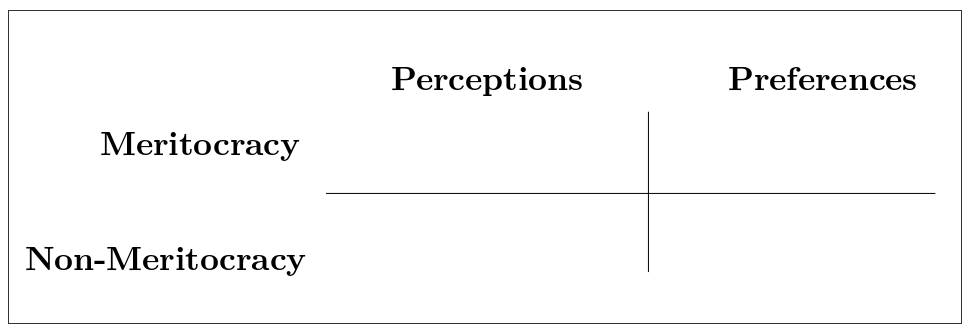
\includegraphics[width=0.85\linewidth]{input/images/Fig1.generalf} 

}

\caption{Conceptual Model of perception and preferences for meritocracy and non-meritocracy}\label{fig:merit-model}
\end{figure}

The columns ``Perceptions'' and ``Preferences'' represent the distinction between these two concepts, usually confused under the label ``beliefs'' (\citeproc{ref-castillo_meritocracia_2019}{Castillo et al., 2019}). Perceptions refer to the extent to which people observe that meritocracy functions or apply in their society, which relates to items such as ``Hard work is important to get ahead in society''. Preferences refer to normative expectations that are frequently linked to a ``should'' expression (e.g.~whether hard work should be related to payment). The rows in Figure \ref{fig:merit-model} consider the distinction between meritocratic and non-meritocratic dimensions (\citeproc{ref-reynolds_perceptions_2014}{Reynolds \& Xian, 2014}), often treated as different ends of the same continuum in previous research. Non-meritocratic elements refer to the use of resources such as personal contacts and/or family advantages to get ahead in life.

The ISSP survey (inequality module) has some items that researchers have used to measure each of the four different dimensions of meritocracy depicted here, but in a rather inconsistent manner. In the next section, we propose a classification of the ISSP meritocracy items into the different dimensions suggested in our multidimensional model depicted in Figure \ref{fig:merit-model} as well as an empirical test of this model.

\section{Methodology}\label{methodology}

The analysis is organized into two studies. The first study is an analysis of the multidimensional model for measuring meritocratic beliefs using ISSP data. Based on the results of this first study, the second study recommends some modifications and expansions of the ISSP items in order to tap better each of the dimensions identified in the study of meritocratic beliefs.

\section{Study 1: Analyzing meritocratic beliefs with ISSP data}\label{study-1-analyzing-meritocratic-beliefs-with-issp-data}

\subsection{Data}\label{data}

The data corresponds to the social inequality module from the International Social Survey Programme (ISSP), the most specialized international comparative survey in perceptions, attitudes, and beliefs about inequality-related issues (\citeproc{ref-issp-research-groupInternationalSocialSurvey2017}{ISSP-Research-Group, 2017}). This wave corresponds to 2009 and covers attitudes towards a series of topics dealing with social inequality across 41 countries and 56,021 individuals. Although there is data available from this module for a more recent wave (2019), the 2009 wave contains relevant items for studying meritocracy that unfortunately are not present in the last wave (details about which items are missing in the last 2019 wave are presented in study 2, Table \ref{tab:table-indicadores}). Table \ref{tab:countries} (appendix) shows details about the sample of countries in the ISSP 2009 data.

\subsection{Variables}\label{variables}

There are a series of indicators in the ISSP survey that we classified in our meritocracy conceptual scheme, as presented below in Table \ref{tab:table-issp}:

\begin{table}[!h]

\caption{\label{tab:table-issp}Items of the ISSP meritocratic perceptions and preferences measures}
\centering
\fontsize{10}{12}\selectfont
\begin{tabular}[t]{>{\raggedright\arraybackslash}p{2cm}>{\raggedright\arraybackslash}p{5cm}>{\raggedright\arraybackslash}p{8cm}}
\toprule
Component & Dimensions & Item\\
\midrule
 &  & How important is having ambition?\\
\cmidrule{3-3}
 & \multirow{-2}{5cm}{\raggedright\arraybackslash Meritocratic} & How important is hard work?\\
\cmidrule{2-3}
 &  & How important is coming from a wealthy family?\\
\cmidrule{3-3}
 &  & How important is having well-educated parents?\\
\cmidrule{3-3}
 &  & How important is a person's race?\\
\cmidrule{3-3}
 &  & How important is being born a man or a woman?\\
\cmidrule{3-3}
 &  & How important is knowing the right people\\
\cmidrule{3-3}
\multirow{-8}{2cm}{\raggedright\arraybackslash Perception} & \multirow{-6}{5cm}{\raggedright\arraybackslash Non-meritocratic} & How important is having political connections\\
\cmidrule{1-3}
 &  & How well he or she does the job?\\
\cmidrule{3-3}
 & \multirow{-2}{5cm}{\raggedright\arraybackslash Meritocratic} & How hard he or she works at the job?\\
\cmidrule{2-3}
 &  & What is needed to support a family?\\
\cmidrule{3-3}
\multirow{-4}{2cm}{\raggedright\arraybackslash Preference} & \multirow{-2}{5cm}{\raggedright\arraybackslash Non-meritocratic} & Whether the person has children to support?\\
\bottomrule
\end{tabular}
\end{table}

\begin{itemize}
\tightlist
\item
  \emph{Perception of meritocracy/non-meritocracy}: for operationalizing perceptions the closest set of ISSP's indicators comes from the question asking about perceptions for opportunities to get ahead, which are usually considered as ``meritocratic beliefs'' in previous studies. The general heading of the battery is: \emph{``To begin we have some questions about opportunities for getting ahead. Please tick one box for each of these to show how important you think it is for getting ahead in life.''} This is followed by a list of statements to be rated from 1 to 5: essential, very important, fairly important, not very important, not important at all.
\end{itemize}

The classification of the items is based on criteria of internal motivation (meritocratic) and structural constraints (non-meritocratic). There were two items from the battery that were excluded from the analysis as they would not fit into the classification. The first one was ``having good education yourself'' since it was not clear whether this could be due to individual motivation or system opportunities, and the second was ``giving bribes'', as introduced elements of criminality that were beyond a non-meritocratic perception.

\begin{itemize}
\tightlist
\item
  \emph{Preferences for meritocracy-non meritocracy}: for the operationalization of normative preferences we used a list of items related to reasons for pay battery. The ISSP question was: \emph{In deciding how much people ought to earn, how important should each of these things be, in your opinion}, rated in the same \emph{essential-non important at all} scale (1 to 5) as the questions for meritocratic perceptions.
\end{itemize}

\subsection{Methods}\label{methods}

The estimation of the measurement model was performed using Confirmatory Factor Analysis (CFA). CFA was conducted using the \texttt{lavaan} R package (version 0.6-3; Rosseel (\citeproc{ref-rosseel_lavaan_2012a}{2012})), with diagonally weighted least squares (DWLS) estimation due to the items' ordinal level of measurement (\citeproc{ref-kline_principles_2016}{Kline, 2016}; \citeproc{ref-rosseel_lavaan_2012a}{Rosseel, 2012}). As recommended by Brown (\citeproc{ref-brown_confirmatory_2015}{2015}), we assessed model fit by jointly considering the comparative fit index and Tucker-Lewis Index (CFI and TLI; acceptable fit \textgreater{} 0.95), Root of the average squared residual approximation (RMSEA; acceptable fit \textless{} 0.08), Chi-square: (p-value; acceptable fit \textgreater{} 0.05, and Chi-square ratio \textgreater{} 3).

\subsection{Results}\label{results}

\subsubsection{Descriptive analyses}\label{descriptive-analyses}

Figure \ref{fig:likert-issp} shows the distribution of responses across the selected items in their corresponding dimensions. On the one side, we observe a high degree of importance attributed to factors such as hard work and ambition for getting ahead, concentrating 94.9\% and 92.8\% in the \emph{fairly important} to \emph{essential} categories, respectively. By contrast, the perception of non-meritocratic aspects is rated lower than the meritocratic ones, particularly for gender, race, and political connections. Regarding normative preferences, we observe that the meritocratic ones are deemed as important (from fairly to essential) for nearly the whole sample, decreasing slightly for the non-meritocratic ones. Still, we have to consider that the preferences for non-meritocratic aspects, in this case, refer to the distributive principle of need rather than personal background (as in the perceptions of non-meritocracy). Such inconsistency between the target of the items for perceptions an preferences is one of the issues to deal with in study 2.

\begin{figure}[H]

{\centering 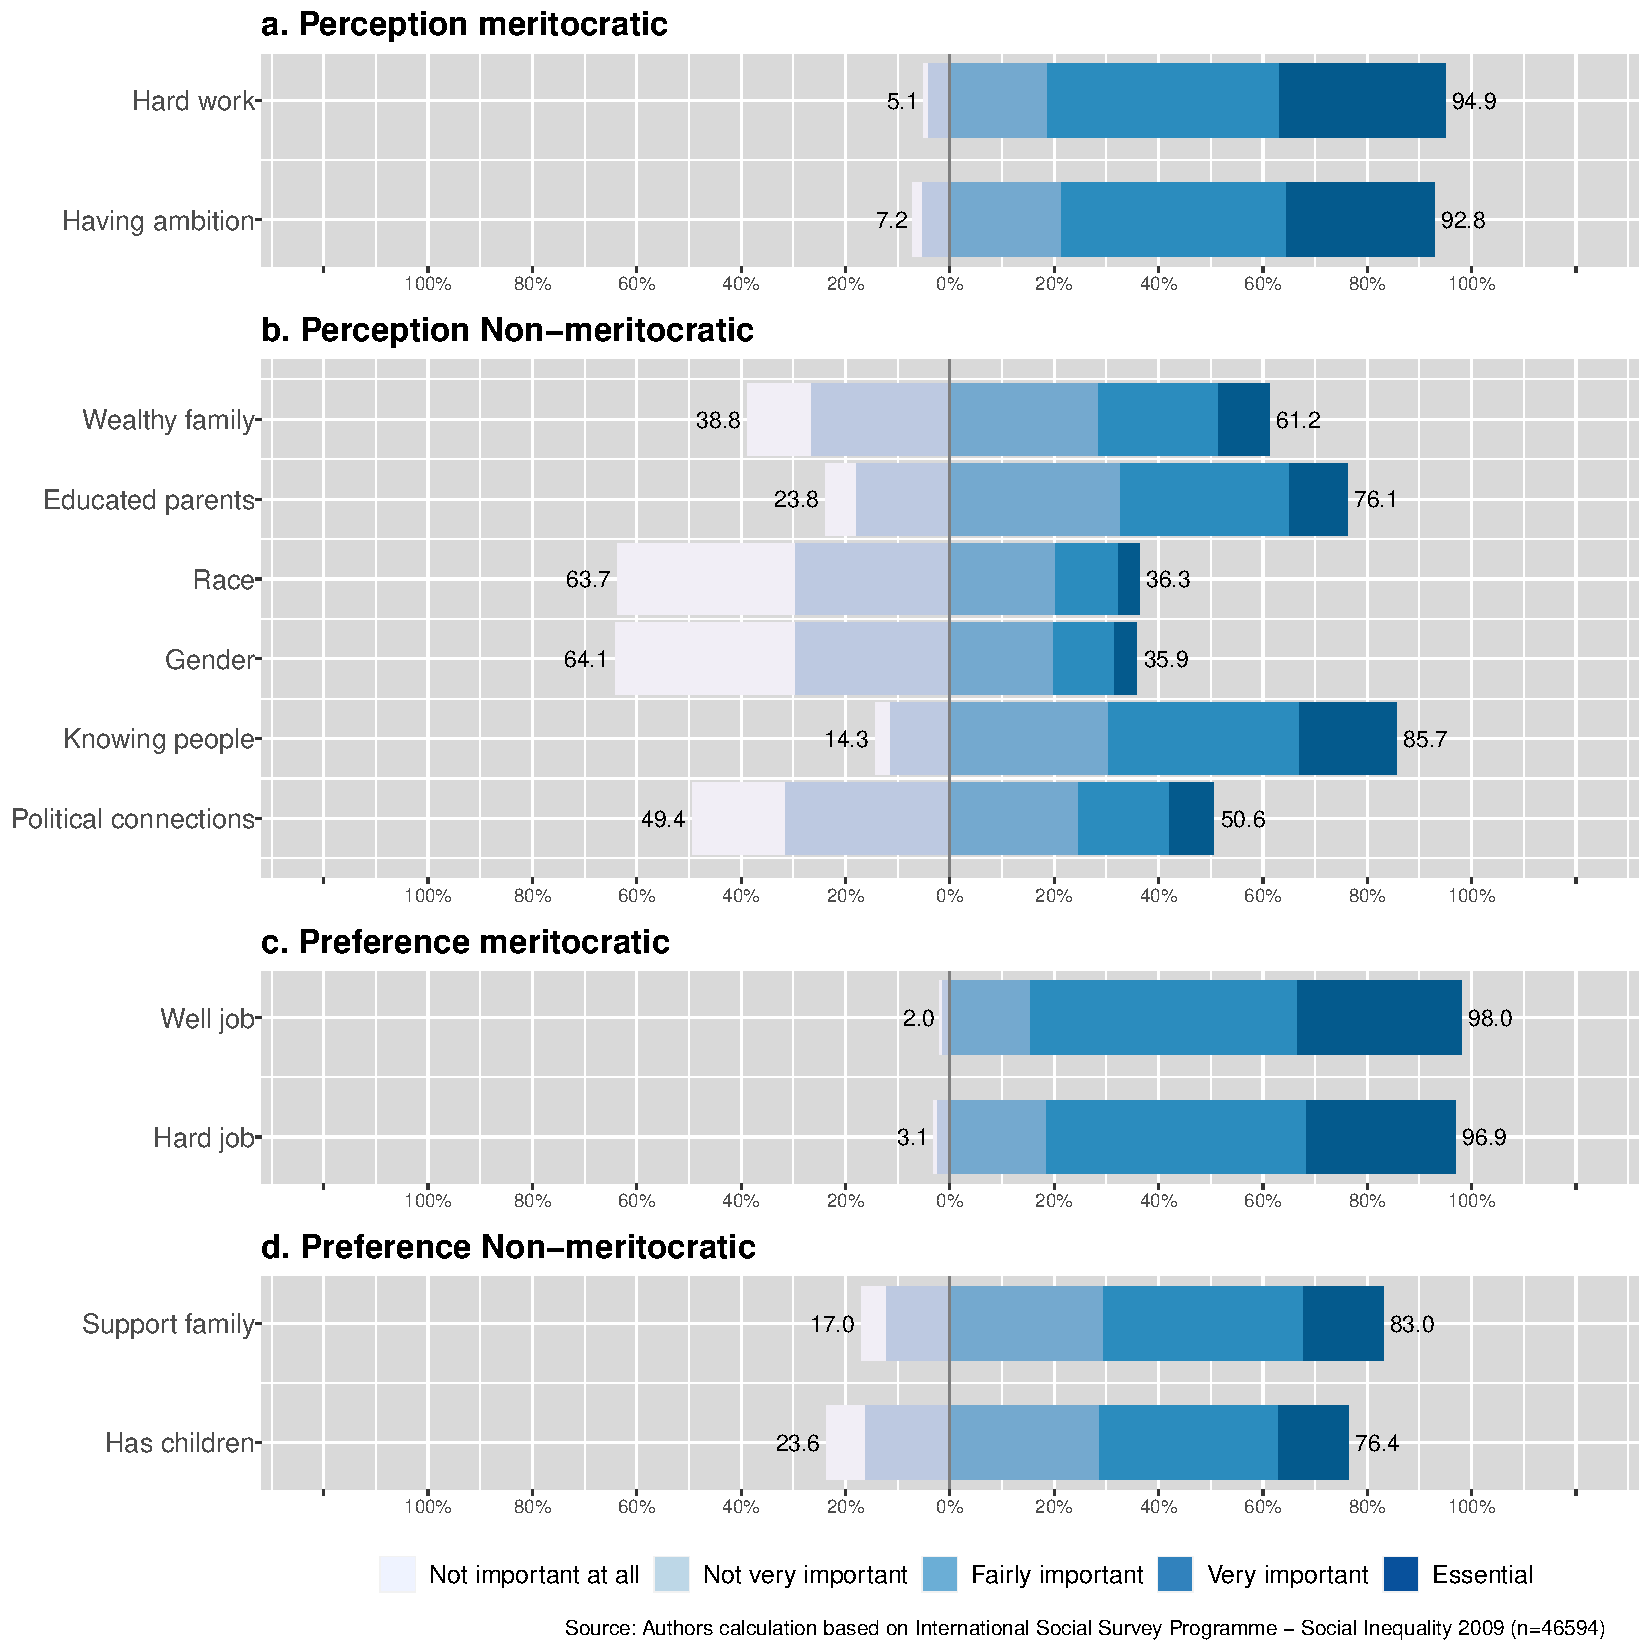
\includegraphics[width=0.8\linewidth]{paper-blinded-RR-IJS_files/figure-latex/likert-issp-1} 

}

\caption{Distribution of responses in the ISSP meritocracy items}\label{fig:likert-issp}
\end{figure}

In terms of the association between the indicators, Figure \ref{fig:corr-issp} shows the polychoric correlation matrix. Firstly, according to the criteria suggested by Cohen (\citeproc{ref-cohen_statistical_1988}{1988}) for effect size, we observe in general that the moderate to high associations are between the pairs of items representing each of the four dimensions described in Table \ref{tab:table-issp}. The exception here is the dimension of non-meritocratic perception, in which six items appear mostly associated by pairs according to their specific topics (family background, personal background, and connections). Still, between this same set of items, moderate correlations could anticipate a single latent factor underlying non-meritocratic perceptions, which is tested next in the confirmatory factor analysis model.

\begin{figure}[H]

{\centering 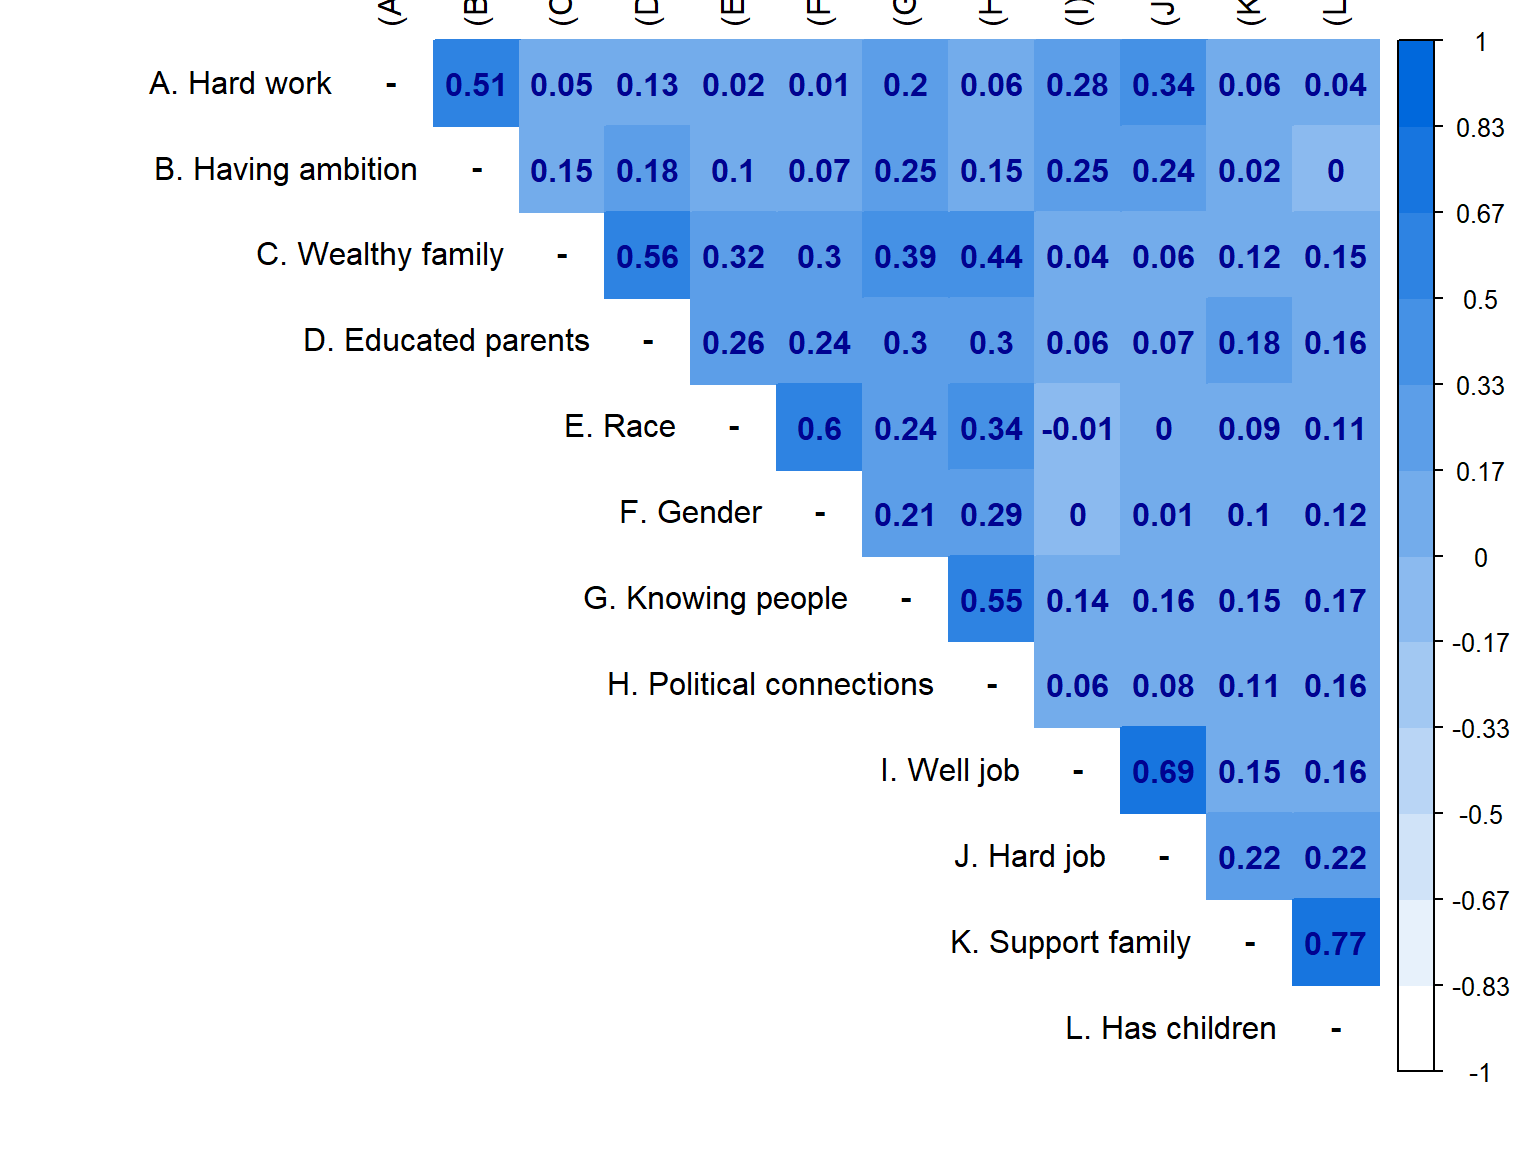
\includegraphics[width=0.85\linewidth]{paper-blinded-RR-IJS_files/figure-latex/corr-issp-1} 

}

\caption{Perceptions and preferences for ISSP  meritocracy items' polychoric correlations}\label{fig:corr-issp}
\end{figure}

\subsubsection{Confirmatory Factor Analysis}\label{confirmatory-factor-analysis}

Table \ref{tab:sum-fit-issp} shows the results of the estimation of two confirmatory models. The first one (First Order) corresponds to a model that estimates four factors, each for one of the dimensions of the multidimensional framework for meritocratic beliefs presented in Table \ref{tab:table-issp}, with only regular fit indicators (CFI=0.959, TLI=0.944, RMSEA=0.098, \(\chi^2\)(df=48)= 21308.535). Further analysis showed that the sources for poor fit were mostly related to the items of the non-meritocratic perceptions, which as mentioned above displayed correlations among them not taken into account in this model specification.

\begin{table}[H]

\caption{\label{tab:sum-fit-issp}Summary fit indices according to model}
\centering
\fontsize{10}{12}\selectfont
\begin{tabular}[t]{lrlrrrrr}
\toprule
Model & $N$ & Estimator & $\chi^2$ & df & CFI & TLI & RMSEA\\
\midrule
First order & 46594 & DWLS & 21308.535 & 48 & 0.959 & 0.944 & 0.098\\
Second order & 46594 & DWLS & 4472.369 & 45 & 0.992 & 0.988 & 0.046\\
\bottomrule
\end{tabular}
\end{table}

Attending to the sources of poor fit from the first estimated confirmatory model, we specified a second model that keeps the basic four-dimensional structure but generates an additional model for the non-meritocratic perceptions as depicted in Figure \ref{fig:meas02-issp}. In this model, the pairs of items in this dimension form three latent factors which at the same time generate a second-order factor of non-meritocratic perceptions, improving the fit of the model significantly.

\begin{figure}[H]

{\centering 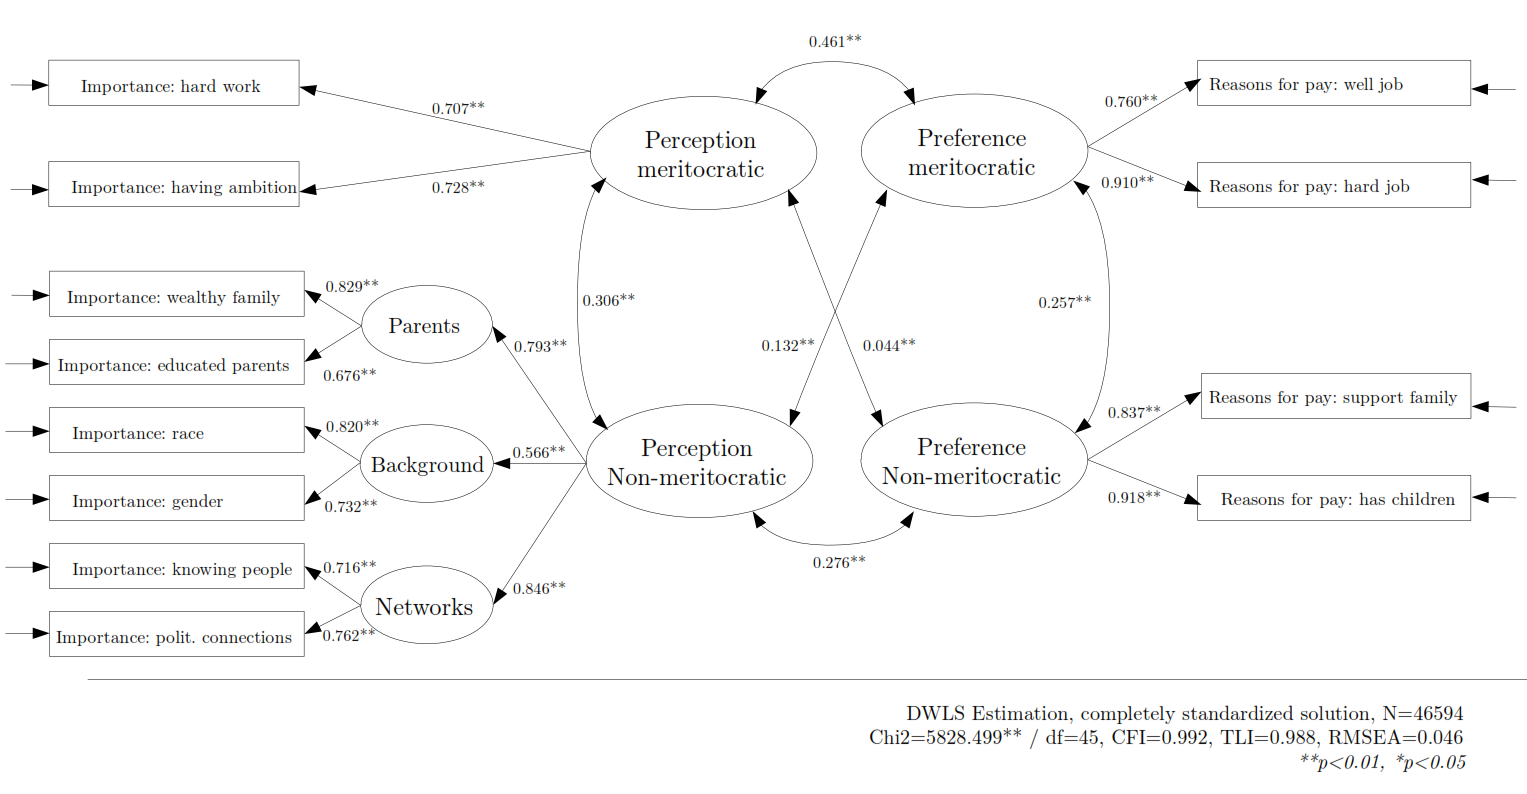
\includegraphics[width=0.85\linewidth]{output/images/figure4} 

}

\caption{Second-order confirmatory factor analysis model using ISSP indicators of Perceptions and Preferences for Meritocracy}\label{fig:meas02-issp}
\end{figure}

Regarding the correlations between the factors in Figure \ref{fig:meas02-issp}, we observe that perceptions are correlated with preferences, but more strongly for the meritocratic (\(r=0.46, p<0.01\)) than for the non-meritocratic (\(r=0.27,p<0.01\)) dimensions. Secondly, both perceptual dimensions (meritocratic and non-meritocratic) depict a moderate positive correlation (\(r=0.30, p<0.01\)), suggesting that they are not the opposite poles of the same continuum as some previous studies assume. Something similar occurs for the correlation between the two dimensions of preferences (\(r=0.25,p<0.01\)).

Based on the previous measurement validation, next we assess some of the potential of the proposed measurement strategy for cross-national comparisons of meritocratic beliefs. In this line, Figure \ref{fig:scat1} depicts the correlation of factor scores for meritocratic perceptions and meritocratic preferences at the country level (\(r=0.65,p<0.01\)). For instance, Bulgaria (BGR) and the United States (USA) appropriately represent the positive association between perception and preferences. In other words, countries that perceived merit in their society as an essential factor to get ahead in life also consider that effort and talent should be determinant factors in how much an individual earns. On the other hand, in countries with lower perceived meritocracy, preferences are also low, where Denmark (DNK) and Venezuela (VEN) are representative cases of this association.

Another finding depicted by Figure \ref{fig:scat1} is the positive association of non-meritocratic perceptions with meritocratic preferences (\(r=0.55,p<0.01\)), showing that countries like Bulgaria (BGR) and Philipines (PHL) represent cases with higher non-meritocratic perceptions and higher preferences for meritocracy. In other words, in societies where people perceive higher importance of non-meritocratic aspects to get ahead in life, people also prefer that merit should be a determinant factor in wages. On the other side, countries like Sweden (SWE) or Denmark (DNK), both Scandinavian societies with strong welfare systems, represent contexts in which non-meritocratic aspects are not described as important, and merit is not considered as a factor that should be relevant for wages. This finding, particularly the positive association between non-meritocratic perception and meritocratic preferences, opens the question of to what extent meritocratic preferences are capable to hold even under evidence of a large amount of perceived non-meritocracy .

\begin{figure}[H]

{\centering 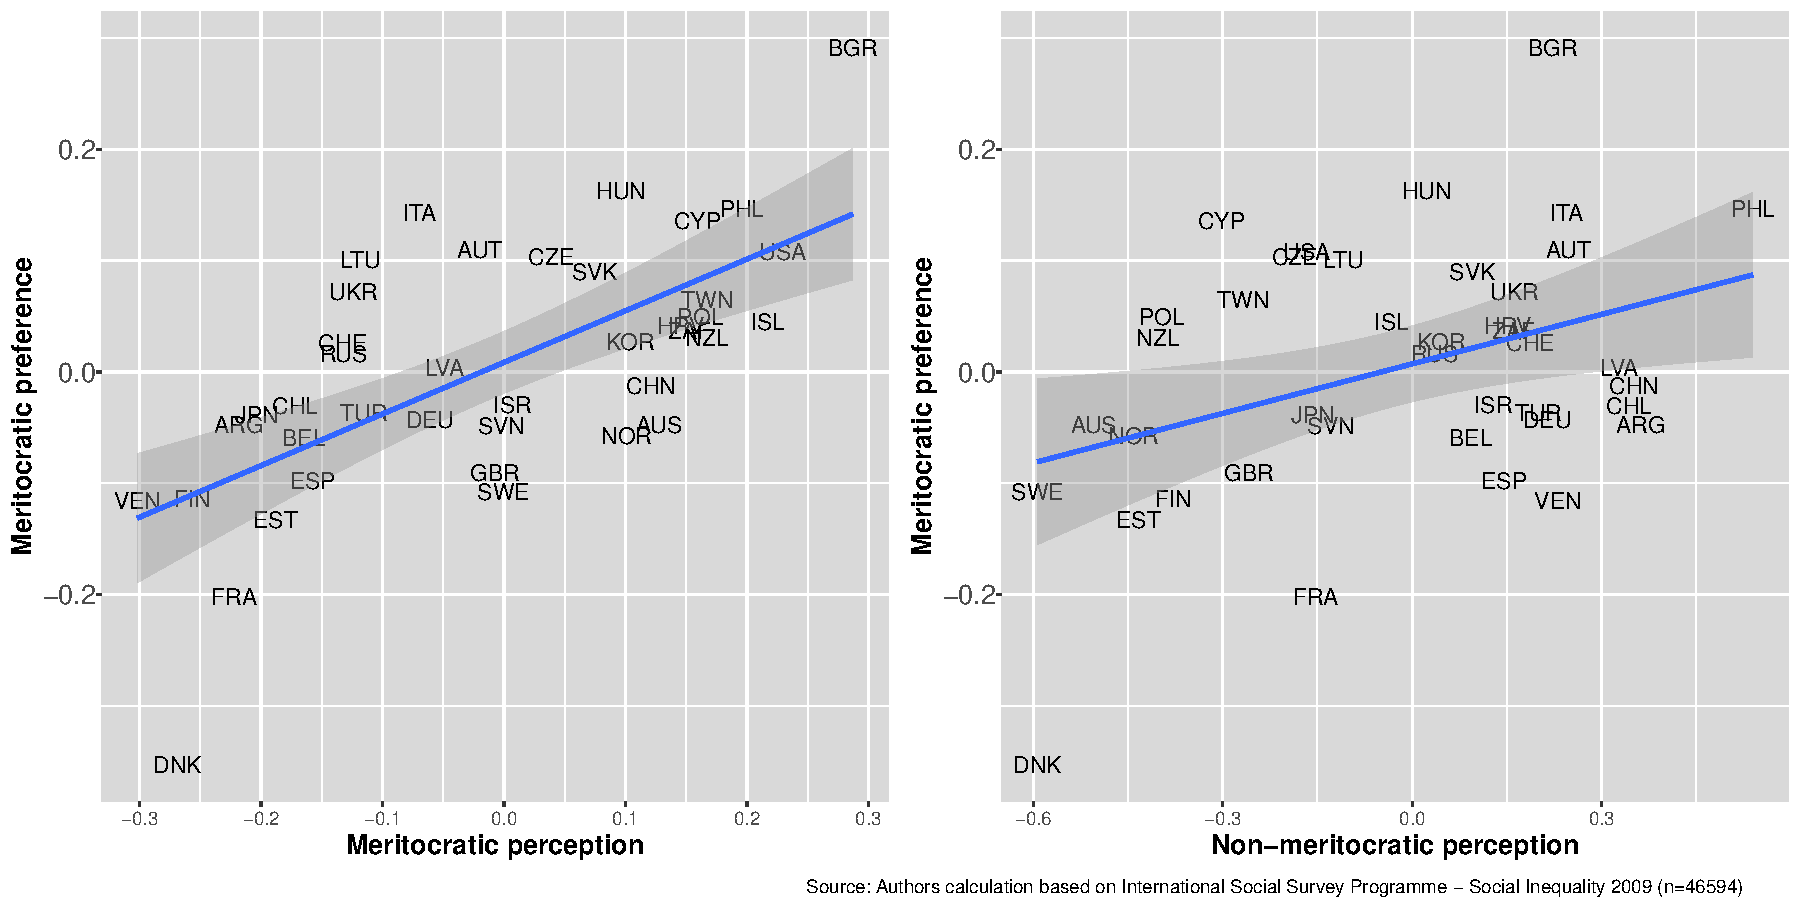
\includegraphics[width=0.85\linewidth]{paper-blinded-RR-IJS_files/figure-latex/scat1-1} 

}

\caption{Cross-national comparison of non-meritocratic and meritocratic perceptions with meritocratic preference}\label{fig:scat1}
\end{figure}

Another possibility to explore within this multidimensional framework of meritocratic beliefs is the differences between countries. For instance, when comparing societies based on their level of industrialization (\citeproc{ref-ishida_trends_2005}{Ishida \& Miwa, 2005}), Figure \ref{fig:scat2} shows that early and late-industrialized countries exhibit a similar association between meritocratic perceptions and preferences (\(r=0.67, p<0.05\); \(r=0.68, p<0.01\), respectively). However, when analyzing the association between non-meritocratic perception and meritocratic preferences, industrialized nations exhibit a strong positive correlation (\(r=0.75, p<0.01\)), which is not the case for late-industrialized countries (\(r=0.29, p>0.05\)). A possible interpretation is that the perception of non-meritocracy in less industrialized societies threatens the meritocratic ideal, which is not the case for the industrialized ones. Still, this preliminary analysis only attempts to show some possiblities that open up when introducing a multidimensional perspective for studying meritocratic beliefs

\begin{figure}[H]

{\centering \includegraphics[width=0.85\linewidth]{paper-blinded-RR-IJS_files/figure-latex/scat2-1} 

}

\caption{Cross-national comparison between industrialized and late-industrialized}\label{fig:scat2}
\end{figure}

\subsection{Discussion Study 1}\label{discussion-study-1}

ISSP is - and probably it will continue to be - the most widely used dataset for comparative studies of meritocratic beliefs. Although several ISSP items were not conceived originally with this end, they have been extensively used to operationalize different aspects of meritocracy. In this study, we ordered and classified ISSP items, which have been previously used for measuring meritocratic beliefs, into four different dimensions: perceptions and preferences, and meritocracy and non-meritocracy. The confirmatory analysis gave evidence of an adequate fit of the multidimensional model to the ISSP data, this is, it is possible to identify perceptions and preferences for meritocracy and non-meritocracy as four related but different constructs. Regarding the non-meritocratic dimensions, we can preliminary conclude that the wide use of reverse-coding for non-meritocratic items attempting to measure meritocratic perceptions or preferences, is not an adequate operationalization. Meritocracy and non-meritocracy are related but different concepts, meaning that it is theoretically possible to find different combinations at individual and contextual levels. This finding opens a series of avenues for future research that are considered in the conclusions.

Despite the advantages of using ISSP data for studying meritocratic beliefs, there are some aspects to be aware of regarding the measurement quality offered by the available items. Some of the items are not really coherent across dimensions, as for instance, meritocratic perceptions are related to ambition and hard work, whereas meritocratic preferences deal with how well a job is done. Such differences impose limitations for a comparative analysis between pereptions and preferences. A better operationalization would require more alignment between the different sides of the same concept, this is, that perceptions and preferences point to the same object of analysis. Furthermore, the instrument is rather unbalanced given the larger amount of non-meritocratic perception items (six) when compared to the number items related to the other dimensions (two). These limitations are taken into account next in the design of study 2.

\section{Study 2: A proposal for a multidimensional measure of meritocratic beliefs}\label{study-2-a-proposal-for-a-multidimensional-measure-of-meritocratic-beliefs}

Taking the analysis of meritocratic beliefs with ISSP as a departing point, the following study offers and test a new measurement instrument that attempts to overcome some limitations identified in the previous study. In this sense, the analysis with ISSP data can be considered as an \emph{inductive} exercise, taking the items and data available and attempting to adjust this information to the proposed multidimensional conceptual model. In the following study we take a complementary \emph{deductive} approach, departing from the conceptual model for the design of a measurement instrument. However, this second approach does not start from scratch, as it is based on ISSP items as much as possible for the sake of comparability with previous studies. The two major differences are: a) it incorporates a balanced and minimalistic representation of items for each of the four dimensions,and b) attempts to maintain the coherence in the topics asked across dimensions (for instance, ``effort'' in items for both perceptions and preferences).

\subsection{Data}\label{data-1}

The data comes from an online survey that was part of a larger study on meritocracy and distributive preferences developed in Chile in 2020, funded by the Chilean National Scientific Agency (ANID). The questionnaire was programmed in Qualtrics and the fieldwork was conducted by an external online survey agency (\href{www.netquest.com}{netquest.com}) between December 2019 and January 2020. The sample was selected from a non-probabilistic quota design in three large cities in Chile (Santiago, Concepción \& Antofagasta). The quotas for gender, age, and educational levels were generated based on a survey by the Public Studies Center (\citeproc{ref-cep_encuesta_2019}{CEP, 2019}), which is a well-regarded counterpart agency of the ISSP (International Social Survey Programme) in Chile. A total sample of 2,141 individuals was collected, excluding those who did not sign the informed consent and those not answering the meritocracy instrument. There were no significant differences between our sample and the wider population for most socio-demographic characteristics, except for the educational level (see Table \ref{tab:rep-samp} in Appendix). As is often the case with online surveys, there were some limitations in achieving the quotas for lower educational levels (\citeproc{ref-boas_recruiting_2020}{Boas et al., 2020}; \citeproc{ref-zhang_quota_2018}{Zhang et al., 2018}). This survey was designed as a three-wave panel and the data used in this analysis corresponds to the first wave.

All participants signed the required informed consent and the survey implementation was approved by the ethical committee from Pontificia Universidad Católica de Chile, protocol ID 150811008, April 6th 2016.

\subsection{Study design}\label{study-design}

\subsubsection{Instrument}\label{instrument}

The proposed items' battery of meritocratic perceptions and preferences consisted of eight indicators, two for each of the four dimensions listed earlier: perceptions (meritocratic/non-meritocratic) and preferences (meritocratic/non-meritocratic). Two main criteria oriented this design. The first one was usability in social survey research, for which the scale length must attend spacer restrictions in such studies. Nevertheless, at the same time, the scale should offer possibilities of accounting for measurement error through factor analysis techniques. Although a rule of thumb in latent measurement suggests at least three indicators per dimension, we still opted for two to count with a brief scale. Although such a decision posits some limitations for modeling measurement error, still allows for factor analysis and is a common approach in previous social survey studies with limited items (for instance see Davidov (\citeproc{ref-davidov_measurement_2009}{2009})). The second criterion is to expand the possibilities of comparability with previous studies on meritocracy, by considering some of the items previously used in this research area. To this regard, some of the items were adapted from the items battery ``reasons to get ahead'' (ISSP/GSS), which has been widely used for operationalizing meritocracy in international research (\citeproc{ref-duru-bellat_who_2012}{Duru-Bellat \& Tenret, 2012}; \citeproc{ref-mijs_paradox_2019}{Mijs, 2019}; \citeproc{ref-reynolds_perceptions_2014}{Reynolds \& Xian, 2014}).

The items, organized according to their respective dimensions, are presented in Table \ref{tab:table-indicadores}. These eight likert-type items have five response alternatives, ranging from ``Completely disagree''(1) to ``Completely agree'' (5). The table presents an additional column with the respective equivalent items from ISSP 2009/2019. With this information it is possible to have a more clear picture of the areas in which the proposed measurement instrument is similar to ISSP and in which ones it differs.

\begin{table}[!h]

\caption{\label{tab:table-indicadores}Items' battery for the multidimensional measurement of meritocratic beliefs and their equivalents in ISSP}
\centering
\fontsize{10}{12}\selectfont
\begin{tabu} to \linewidth {>{\raggedright\arraybackslash}p{1.5cm}>{\raggedright\arraybackslash}p{2 cm}>{\raggedright}X>{\raggedright}X}
\toprule
Component & Dimensions & Items & Items ISSP (2009,2019)\\
\midrule
 &  & Those who make more effort get greater rewards than those who make less effort. & How important is hard work?\\
\cmidrule{3-4}
 & \multirow{-2}{2 cm}{\raggedright\arraybackslash Meritocratic} & Those with more talent get greater rewards than those who have less talent. & -\\
\cmidrule{2-4}
 &  & Those who have rich parents manage to get ahead. & How important is coming from a wealthy family?\\
\cmidrule{3-4}
\multirow{-4}{1.5cm}{\raggedright\arraybackslash Perception} & \multirow{-2}{2 cm}{\raggedright\arraybackslash Non meritocratic} & Those who have good contacts manage to get ahead. & How important is knowing the right people\\
\cmidrule{1-4}
 &  & Those who make more effort should get greater rewards than those who make less effort. & How hard he or she works at the job?*\\
\cmidrule{3-4}
 & \multirow{-2}{2 cm}{\raggedright\arraybackslash Meritocratic} & Those who have more talent should get greater rewards than those who have less talent. & How well he or she does the job?*\\
\cmidrule{2-4}
 &  & It is fine if those with rich parents get ahead. & -\\
\cmidrule{3-4}
\multirow{-4}{1.5cm}{\raggedright\arraybackslash Preference} & \multirow{-2}{2 cm}{\raggedright\arraybackslash Non meritocratic} & It is fine if those with good contacts get ahead. & -\\
\bottomrule
\multicolumn{4}{l}{\rule{0pt}{1em}\textit{Note: } Those with an asterisk (*) are only present in 2009}\\
\end{tabu}
\end{table}
\pagebreak

\subsubsection{Administration sets}\label{administration-sets}

To evaluate the effect of indicator ordering in the responses, three different versions of items' order were designed and randomly assigned to the respondents, as depicted in Figure \ref{fig:appmod}. The scale was presented to the first group (\emph{n = 712}) in the order shown in Table \ref{tab:table-indicadores} according to perceptions and preferences. For the second group (\emph{n = 717}), the order was reorganized according to perceptions and preferences over the same topic, e.g., for the topic of hard work, the item about perception was followed by the item about preference and the same for the rest of the topics. Finally, for the third group (\emph{n = 712}), the items were presented as completely randomized.

\begin{figure}[H]

{\centering 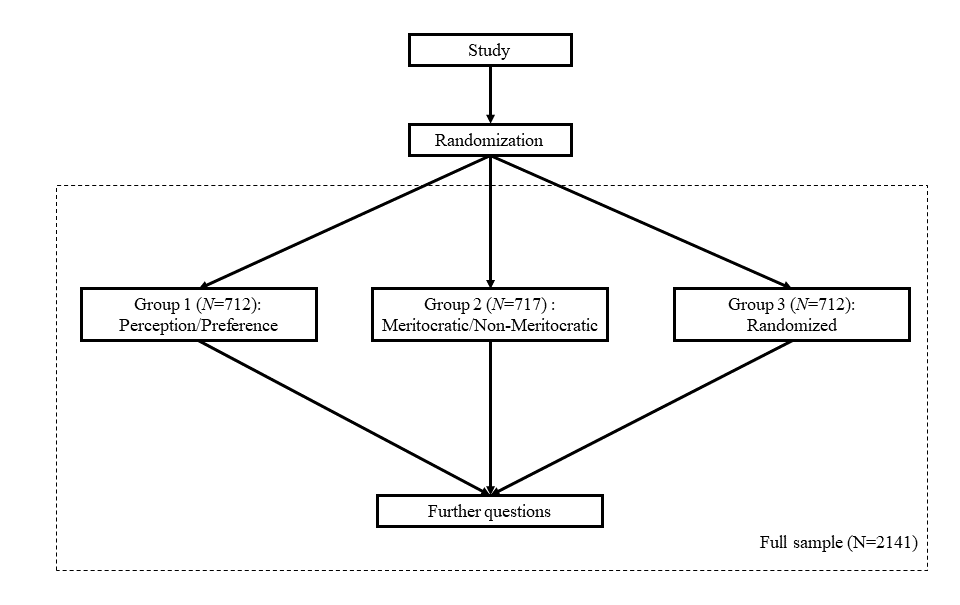
\includegraphics[width=0.85\linewidth]{output/images/figure6} 

}

\caption{Survey flow}\label{fig:appmod}
\end{figure}

\subsection{Methods}\label{methods-1}

To test the scale's underlying constructs, we employed confirmatory factor analysis models (CFA). The models estimated one factor for each of the four proposed dimensions presented in Table \ref{tab:table-indicadores}. As in study 1, CFA was performed with the \texttt{lavaan} R package (version 0.6-3; Rosseel (\citeproc{ref-rosseel_lavaan_2012a}{2012})), with diagonally weighted least squares (DWLS) estimation due to the items' ordinal level of measurement (\citeproc{ref-kline_principles_2016}{Kline, 2016}; \citeproc{ref-rosseel_lavaan_2012a}{Rosseel, 2012}). The fit indexes and cut-off criteria were the same as the ones used in Study 1.

A pre-registration was made in the OSF platform, available at the following link: \href{https://osf.io/z45y2/?view_only=adcd496887f2471597b1d6ffb46e492d}{https://osf.io/z45y2}. This pre-registration includes the hypotheses regarding the four-dimensional conceptual model underlying the scale, the variable measurement levels, the statistical tests to be performed with their respective evaluation parameters, and other important aspects of the research design.

\subsection{Results}\label{results-1}

\subsubsection{Descriptive analyses}\label{descriptive-analyses-1}

The graphs presented in Figure \ref{fig:plotlikert} display disaggregated and comparable information of the different response categories for each item. Generally, there is more agreement in the perception of non-meritocratic items than in meritocratic ones, while in the preferences, the opposite occurs. Regarding preferences, the predominant role of effort over talent as a criterion of meritocratic preference is noteworthy. All in all, the descriptive results show a critical view of meritocracy, perceiving the operation of non-meritocratic aspects over meritocratic ones, whereas in the preferences the opposite occurs.

\begin{figure}[H]

{\centering 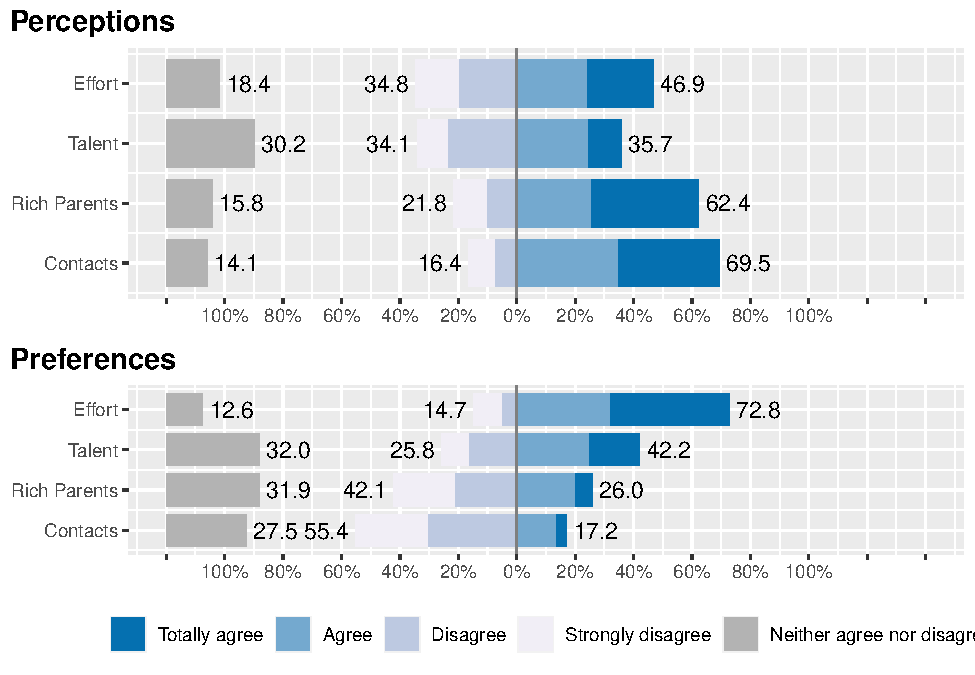
\includegraphics[width=0.85\linewidth]{paper-blinded-RR-IJS_files/figure-latex/plotlikert-1} 

}

\caption{Distribution of responses in the Merit Scale items}\label{fig:plotlikert}
\end{figure}

Attending now to the association among the scale items, Figure \ref{fig:corpoly} shows the items' polychoric correlations. There are three main aspects to highlight from this correlation matrix. Firstly, and as expected, the largest correlations are between indicators that correspond to the same factors (dimensions) behind the conceptual model (e.g., perception of meritocracy by effort and by talent, \(r=0.52,p<0.01\)). Secondly, among these correlations, the highest are those between the non-meritocratic dimensions, both in perceptions (\(r=0.73,p<0.01\)) and preferences (\(r=0.61,p<0.01\)). Thirdly, both items for meritocratic preferences (E and F) are the ones that mostly correlate with the rest of the perceptual items, showing medium to high correlations and indicating that the perception of non-meritocracy would be related to larger meritocratic preferences. Finally, similar to the results of study 1 with ISSP data, we observe no considerable negative correlations between meritocratic and non-meritocratic aspects, undermining previous studies' assumptions that these dimensions would be the opposite poles of one same continuum (\citeproc{ref-reynolds_perceptions_2014}{Reynolds \& Xian, 2014}).

\begin{figure}[H]

{\centering 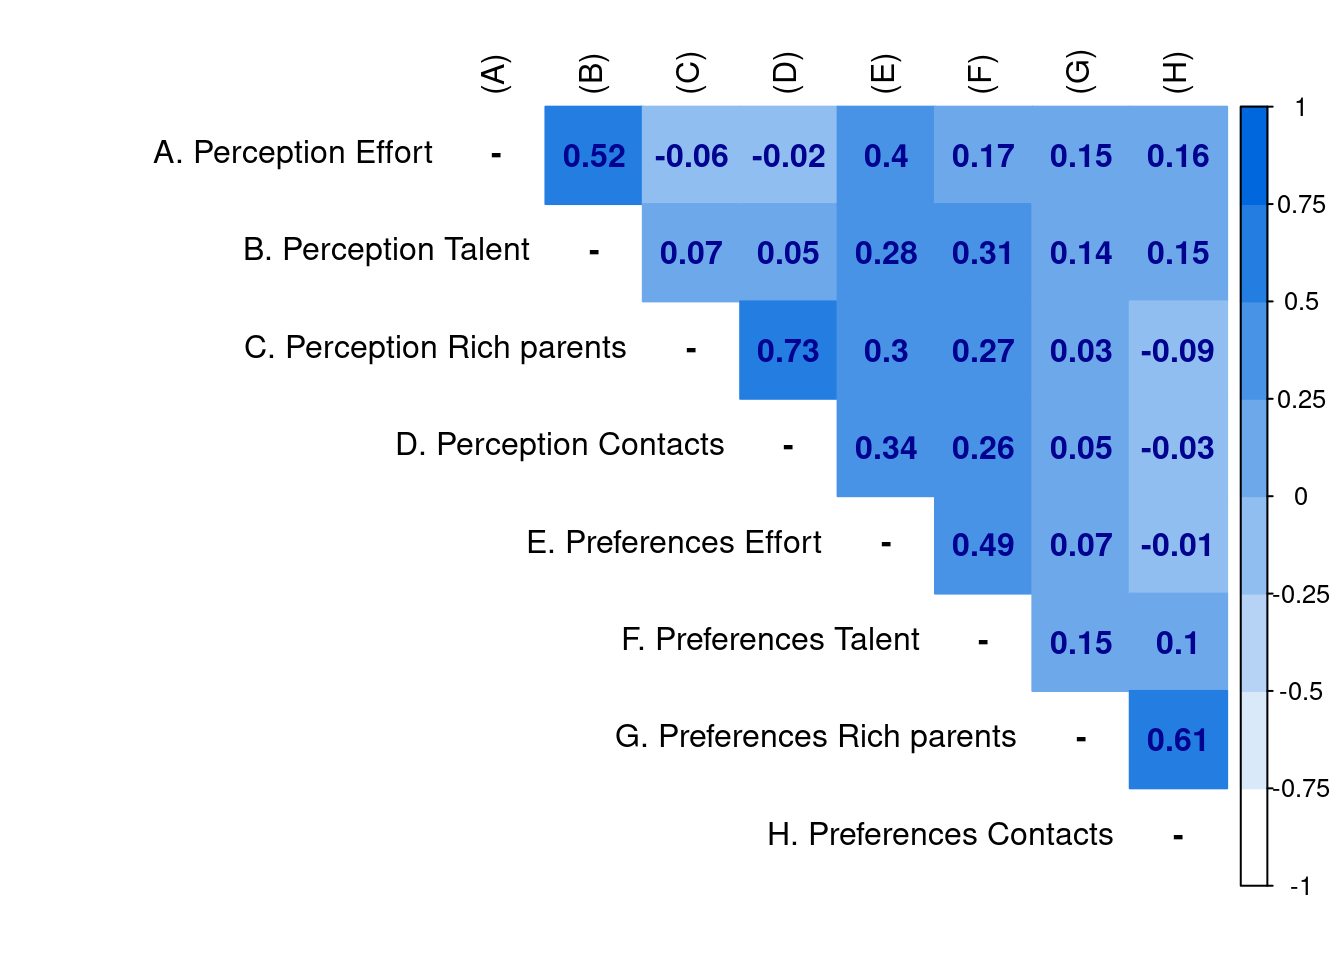
\includegraphics[width=0.85\linewidth]{paper-blinded-RR-IJS_files/figure-latex/corpoly-1} 

}

\caption{Perceptions and preferences for meritocracy items' polychoric correlations}\label{fig:corpoly}
\end{figure}

\subsubsection{Confirmatory Factor Analysis}\label{confirmatory-factor-analysis-1}

The present section describes the results of the confirmatory factor analysis estimation. The model estimates four latent factors: perception meritocratic, perception non-meritocratic, preferences meritocratic, and preferences non-meritocratic. Each factor is estimated based on two scale items as detailed in Table \ref{tab:table-indicadores}.

The first step in the analysis consists of comparing the model fit indicators for the three versions of the instrument that were randomly assigned to the participants: order according to perceptions/preferences, order according to topics, and a complete random items' order (see Figure \ref{fig:appmod}).

\begin{table}[H]

\caption{\label{tab:table-cfafits}Summary fit indices according to order versions}
\centering
\fontsize{10}{12}\selectfont
\begin{tabular}[t]{lrlrrrrr}
\toprule
Model & $N$ & Estimator & $\chi^2$ & df & CFI & TLI & RMSEA\\
\midrule
Version 1 & 712 & DWLS & 25.631 & 14 & 0.998 & 0.996 & 0.034\\
Version 2 & 717 & DWLS & 67.652 & 14 & 0.984 & 0.967 & 0.073\\
Version 3 & 712 & DWLS & 41.633 & 14 & 0.991 & 0.981 & 0.053\\
\bottomrule
\end{tabular}
\end{table}

Table \ref{tab:table-cfafits} shows the fit indicators of the models estimated for each of the three versions of the items' order described in the methodology. Regardless of the version, all models obtained adequate fit indicators, with CFI's above 0.95 and RMSEA's below 0.08. However, none of the models achieved a non-significant chi-square, as expected in large samples like the one used here. The first version order (perceptions-preferences) was the one obtaining the best fit (CFI=0.993, TLI=0.995, RMSEA=0.034, \(\chi2\)(df=14)=42.276), whereas version 2 with the fixed order according to merit/non-merit items shows the comparatively worst indicators. The CFA fit indices for the completely randomized items' order (Model 3) keep all the indicators within the acceptable cut-off criteria and controls for possible order effects in the administration of the instrument. The model and parameter estimates for this version are depicted in Figure \ref{fig:meas02}:

\begin{figure}[H]

{\centering 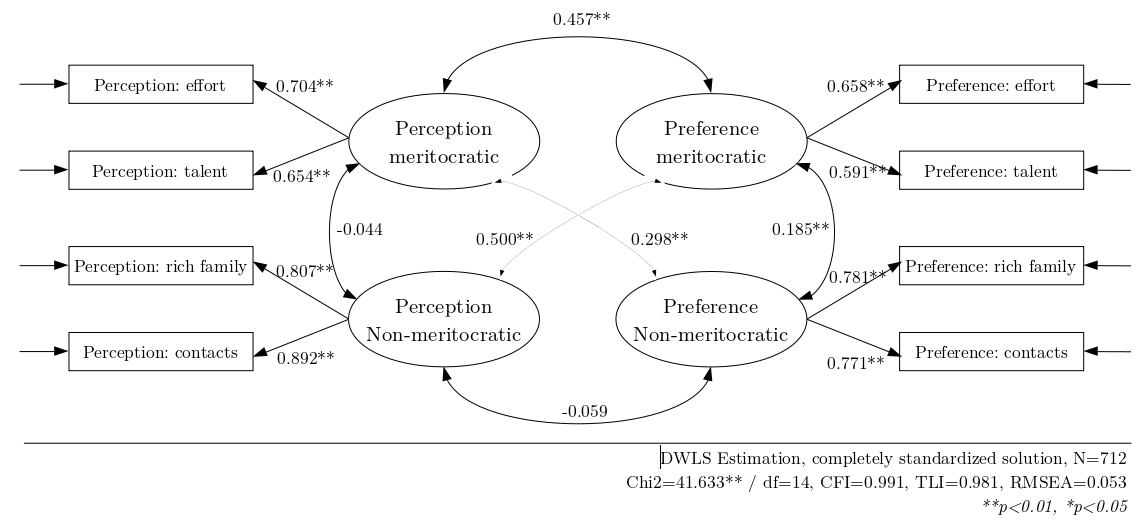
\includegraphics[width=0.85\linewidth]{output/images/figure9} 

}

\caption{Confirmatory factor analysis of the Perceptions and Preferences for Meritocracy Scale}\label{fig:meas02}
\end{figure}

Attending to the correlations between the latent variables as depicted in Figure \ref{fig:meas02}, meritocratic preferences are moderate to highly correlated with perceptions, both meritocratic (\(r=0.457,p<0.01\)) and non-meritocratic (\(r=0.500,p<0.01\)). The correlation between both types of perceptions (\(r=-0.044,p>0.05\)) and both types of preferences (\(r=0.185,p<0.01\)) was low, as well as between non-meritocratic preferences and perceptions (\(r=-0.059p>0.05\)). This last finding gives further evidence regarding the lack of unidimensionality of meritocratic and non-meritocratic aspects as assumed by previous studies.

The measurement of meritocratic beliefs with this new instrument shows, in general, better fit - and therefore better measurement quality - than study 1. However, the comparison between the two studies is unbalanced as we are comparing one particular country (study 2) with the whole set of ISSP countries (study 1). To clear this point, we performed an additional analysis of ISSP data only for the case of Chile. Overall, the results for the chilean ISSP data show a similar fit to the ones of with the complete ISSP dataset (CFI=0.987, TLI=0.980, RMSEA=0.055, \(\chi^2\)(df=45)= 234), and therefore the instrument of study 2 outperforms their fit indicators.

\subsection{Discussion Study 2}\label{discussion-study-2}

The eight-items' battery presented here and the estimation of the confirmatory model with chilean data gives additional evidence for a multidimensional concept of meritocratic beliefs. Despite the good general working of the scale, there are some limitations in interpreting the results given the few items (two) per dimension. As mentioned before, the option of a minimalistic approach in terms of items has advantages and disadvantages: advantages in terms of usability in social surveys with limited space and disadvantages in terms of measurement validity in the estimation of the latent constructs. Regarding the practical use of the measurement instruments, the primary lesson from our study 2 is the importance of distinguishing between the four dimensions. We recommend using the eight-items battery when scholars intend to measure both perceptions and preferences. Alternatively, scholars can use the individual components separately. For instance, researchers interested in the dimension of perception can use only the four items that assess both the meritocratic and non-meritocratic perception. Furthermore, this measurement proposal can be used for relating the dimensions among themselves (for instance, to what extent the perception of meritocracy is related to the preference of it). It can also serve to studies about how each of these dimensions is associated with or moderated by individual and country level variables.

\section{Conclusions}\label{conclusions}

Studies that attempt to characterize and compare societies by their support for meritocratic beliefs have used different approaches. As most studies use secondary survey data, and by and large items from the social inequality module from ISSP, they tend to assume that the available indicators represent an underlying meritocratic construct. A review of these studies reveals several non-tested assumptions and the use of similar indicators to represent different constructs and dimensions of meritocracy. As the existence of heterogeneous approaches certainly has consequences for the advancement of the study of meritocracy, this paper presented a comprehensive multidimensional conceptual framework for the empirical study of meritocracy, building upon previous research. We tested the validity of our conceptual framework with two studies. In a first study, this framework was operationalized and tested with ISSP international data. Based on the results with ISSP, a second study proposed some improvements to the measure of meritocracy with ISSP, which was tested with novel data from a single country case (Chile).

The results of our empirical studies show evidence in favor of a four dimensional model of meritocracy, opening interesting avenues for future comparative research. For instance, distinguishing perceptions from preferences will allow us to evaluate the extent to which different societies are accustomed to, or satisfied with, the perceived level of meritocracy, in terms of differences between what is perceived and what is preferred. Additionally, given that non-meritocratic factors are not necessarily related to meritocratic ones, the multidimensional measurement of meritocratic beliefs makes it possible to assess the perceived legitimacy of practices such as the use of personal contacts and their interference (or not) with meritocratic ideals in different societies. Considering how individual and societal structural factors are related to meritocracy will allow us to gain knowledge about the legitimacy of distribution based on meritocratic criteria. Furthermore, the impact of different configurations of the four-dimensional framework on practices and behaviors, such as corruption, civic involvement, and political alignment, are areas that open up for future development. Such agendas could be especially relevant in times of economic crisis and growing inequalities, which could entail changes in the legitimation of the current distributive structure based on meritocratic ideals.

Besides the areas of research with comparative survey studies as ISSP, single case studies as well as future comparative studies (ISSP included) might benefit from taking into account the measurement instrument for meritocracy proposed here, tested so far with novel Chilean data. The instrument is to some extent comparable to ISSP - as some of its items are equivalent - but improves the balanced measurement of the four dimensions in a minimalistic eight-items' battery, suitable for survey research. Still, further evidence is needed in order to assess the external validity of the results. Upcoming research in the area of meritocratic beliefs, a growing research agenda, would certainly help to keep improving the quality of the measurement instruments in this area, which is a key enterprise when it comes to assess the support and legitimacy of the meritocratic distribution, particularly in unequal societies.

\section{Transparency statement}\label{transparency-statement}

This research follows a series of open science guidelines as the pre-registration of Study 2 (scale development) as well as the availability of data and codes (R) in a public repository in Github. This document was generated with the R package Rmarkdown and contains the code for all the tables and figures to make it reproducible.

\section{References}\label{references}

\phantomsection\label{refs}
\begin{CSLReferences}{1}{0}
\bibitem[\citeproctext]{ref-aiello_new_2019}
Aiello, F., Cardamone, P., \& Pupo, V. (2019). New evidence on the firm-university linkages in {Europe}. {The} role of meritocratic management practices. \emph{International Review of Applied Economics}, \emph{33}(6), 813--828. \url{https://doi.org/10.1080/02692171.2019.1608917}

\bibitem[\citeproctext]{ref-alesina_fairness_2005}
Alesina, A., \& Angeletos, G. (2005). Fairness and redistribution. \emph{American Economic Review}, 960--980.

\bibitem[\citeproctext]{ref-ansolabehere_strength_2008}
Ansolabehere, S., Rodden, J., \& Snyder, J. M. (2008). The {Strength} of {Issues}: {Using Multiple Measures} to {Gauge Preference Stability}, {Ideological Constraint}, and {Issue Voting}. \emph{American Political Science Review}, \emph{102}(2), 215--232. \url{https://doi.org/10.1017/S0003055408080210}

\bibitem[\citeproctext]{ref-arrow_meritocracy_2000}
Arrow, K. J., Bowles, S., \& Durlauf, S. N. (Eds.). (2000). \emph{Meritocracy and economic inequality}. {Princeton University Press}.

\bibitem[\citeproctext]{ref-atria_economic_2020}
Atria, J., Castillo, J., Maldonado, L., \& Ramirez, S. (2020). Economic {Elites}' {Attitudes Toward Meritocracy} in {Chile}: {A Moral Economy Perspective}. \emph{American Behavioral Scientist}, \emph{64}(9), 1219--1241. \url{https://doi.org/10.1177/0002764220941214}

\bibitem[\citeproctext]{ref-boas_recruiting_2020}
Boas, T. C., Christenson, D. P., \& Glick, D. M. (2020). Recruiting large online samples in the {United States} and {India}: {Facebook}, {Mechanical Turk}, and {Qualtrics}. \emph{Political Science Research and Methods}, \emph{8}(2), 232--250. \url{https://doi.org/10.1017/psrm.2018.28}

\bibitem[\citeproctext]{ref-bollen_structural_1989}
Bollen, K. A. (1989). \emph{Structural equations with latent variables}. {Wiley}.

\bibitem[\citeproctext]{ref-breen_class_1999}
Breen, R., \& Goldthorpe, J. H. (1999). Class inequality and meritocracy: A critique of {Saunders} and an alternative analysis. \emph{The British Journal of Sociology}, \emph{50}(1), 1--27. \url{https://doi.org/10.1111/j.1468-4446.1999.00001.x}

\bibitem[\citeproctext]{ref-brown_confirmatory_2015}
Brown, T. (2015). \emph{Confirmatory factor analysis for applied research} (Second edition). {The Guilford Press}.

\bibitem[\citeproctext]{ref-bubak_perceptions_2019}
Bubak, O. (2019). Perceptions of meritocracy: {A} note on {China}. \emph{Asian Journal of Comparative Politics}, \emph{4}(2), 192--209. \url{https://doi.org/10.1177/2057891118806065}

\bibitem[\citeproctext]{ref-castillo_meritocracia_2019}
Castillo, J. C., Torres, A., Atria, J., \& Maldonado, L. (2019). Meritocracia y desigualdad económica: {Percepciones}, preferencias e implicancias. \emph{Revista Internacional de Sociología}, \emph{77}(1), 117. \url{https://doi.org/10.3989/ris.2019.77.1.17.114}

\bibitem[\citeproctext]{ref-cep_encuesta_2019}
CEP. (2019). \emph{Encuesta {CEP Mayo} 2019}.

\bibitem[\citeproctext]{ref-chen_sensitivity_2007}
Chen, F. F. (2007). Sensitivity of {Goodness} of {Fit Indexes} to {Lack} of {Measurement Invariance}. \emph{Structural Equation Modeling: A Multidisciplinary Journal}, \emph{14}(3), 464--504. \url{https://doi.org/10.1080/10705510701301834}

\bibitem[\citeproctext]{ref-cheung_evaluating_2002}
Cheung, G. W., \& Rensvold, R. B. (2002). Evaluating {Goodness-of-Fit Indexes} for {Testing Measurement Invariance}. \emph{Structural Equation Modeling: A Multidisciplinary Journal}, \emph{9}(2), 233--255. \url{https://doi.org/10.1207/S15328007SEM0902_5}

\bibitem[\citeproctext]{ref-cohen_statistical_1988}
Cohen, J. (1988). \emph{Statistical power analysis for the behavioral sciences} (2nd ed). {L. Erlbaum Associates}.

\bibitem[\citeproctext]{ref-converse_nature_1964}
Converse, P. E. (1964). The nature of belief systems in mass publics (1964). \emph{Critical Review}, \emph{18}(1-3), 1--74. \url{https://doi.org/10.1080/08913810608443650}

\bibitem[\citeproctext]{ref-davey_preference_1999}
Davey, L. M., Bobocel, D. R., Son Hing, L. S., \& Zanna, M. P. (1999). Preference for the {Merit Principle Scale}: {An} individual difference measure of distributive justice preferences. \emph{Social Justice Research}, \emph{12}(3), 223--240.

\bibitem[\citeproctext]{ref-davidov_measurement_2009}
Davidov, E. (2009). Measurement {Equivalence} of {Nationalism} and {Constructive Patriotism} in the {ISSP}: 34 {Countries} in a {Comparative Perspective}. \emph{Political Analysis}, \emph{17}(1), 64--82. \url{https://doi.org/10.1093/pan/mpn014}

\bibitem[\citeproctext]{ref-davidov_measurement_2014}
Davidov, E., Meuleman, B., Cieciuch, J., Schmidt, P., \& Billiet, J. (2014). Measurement {Equivalence} in {Cross-National Research}. \emph{Annual Review of Sociology}, \emph{40}(1), 55--75. \url{https://doi.org/10.1146/annurev-soc-071913-043137}

\bibitem[\citeproctext]{ref-dimick_models_2018}
Dimick, M., Rueda, D., \& Stegmueller, D. (2018). Models of other-regarding preferences, inequality, and redistribution. \emph{Annual Review of Political Science}, \emph{21}(1), 441--460. \url{https://doi.org/10.1146/annurev-polisci-091515-030034}

\bibitem[\citeproctext]{ref-dimitrov_testing_2010}
Dimitrov, D. M. (2010). Testing for {Factorial Invariance} in the {Context} of {Construct Validation}. \emph{Measurement and Evaluation in Counseling and Development}, \emph{43}(2), 121--149. \url{https://doi.org/10.1177/0748175610373459}

\bibitem[\citeproctext]{ref-duru-bellat_who_2012}
Duru-Bellat, M., \& Tenret, E. (2012). Who's for meritocracy? {Individual} and contextual variations in the faith. \emph{Comparative Education Review}, \emph{56}(2), 223--247. \url{https://doi.org/10.1086/661290}

\bibitem[\citeproctext]{ref-fischer_are_2011}
Fischer, R., Ferreira, M. C., Jiang, D.-Y., Cheng, B.-S., Achoui, M. M., Wong, C. C., Baris, G., Mendoza, S., van Meurs, N., Achmadi, D., Hassan, A., Zeytinoglu, G., Dalyan, F., Harb, C., Darwish, D. D., \& Assmar, E. M. (2011). Are {Perceptions} of {Organizational Justice Universal}? {An Exploration} of {Measurement Invariance Across Thirteen Cultures}. \emph{Social Justice Research}, \emph{24}(4), 297--313. \url{https://doi.org/10.1007/s11211-011-0142-7}

\bibitem[\citeproctext]{ref-generett_stories_2020}
Generett, G. G., \& Olson, A. M. (2020). The stories we tell: {How} merit narratives undermine success for urban youth. \emph{Urban Education}, \emph{55}(3), 394--423. \url{https://doi.org/10.1177/0042085918817342}

\bibitem[\citeproctext]{ref-girerd_neoliberalism_2020}
Girerd, L., \& Bonnot, V. (2020). Neoliberalism: {An} ideological barrier to feminist identification and collective action. \emph{Social Justice Research}, \emph{33}(1), 81--109. \url{https://doi.org/10.1007/s11211-020-00347-8}

\bibitem[\citeproctext]{ref-goldthorpe_myth_2003}
Goldthorpe, J. (2003). The myth of education-based meritocracy. \emph{New Economy}, \emph{10}(4), 234--239. \url{https://doi.org/10.1046/j.1468-0041.2003.00324.x}

\bibitem[\citeproctext]{ref-hadjar_meritokratie_2008}
Hadjar, A. (2008). \emph{Meritokratie als legitimationsprinzip}. {VS Verlag}.

\bibitem[\citeproctext]{ref-ishida_trends_2005}
Ishida, H., \& Miwa, S. (2005). Trends in intergenerational class mobility and education in japan. \emph{Social Stratification and Social Mobility in Late-Industrializing Countries}.

\bibitem[\citeproctext]{ref-issp-research-groupInternationalSocialSurvey2017}
ISSP-Research-Group. (2017). \emph{International {Social Survey Programme}: {Social Inequality Dataset IV} - {ISSP} 2009}. {GESIS Data Archive}. \url{https://doi.org/10.4232/1.12777}

\bibitem[\citeproctext]{ref-janmaat_subjective_2013}
Janmaat, J. G. (2013). Subjective inequality: A review of international comparative studies on people's views about inequality. \emph{European Journal of Sociology}, \emph{54}(3), 357--389. \url{https://doi.org/10.1017/S0003975613000209}

\bibitem[\citeproctext]{ref-khan_privilege_2013}
Khan, S. (2013). \emph{Privilege: {The} making of an adolescent elite at st. {Paul}'s school} (first paperback printing). {Princeton Univ. Press}.

\bibitem[\citeproctext]{ref-kline_principles_2016}
Kline, R. B. (2016). \emph{Principles and practice of structural equation modeling, 4th ed.} (pp. xvii, 534). {Guilford Press}.

\bibitem[\citeproctext]{ref-kluegel_beliefs_1986}
Kluegel, J. R., \& Smith, E. R. (1986). \emph{Beliefs about {Inequality}: {Americans}' {Views} of {What Is} and {What Ought} to {Be}} (First). {Routledge}. \url{https://doi.org/10.4324/9781351329002}

\bibitem[\citeproctext]{ref-kunovich_systems_2007}
Kunovich, S., \& Slomczynski, K. M. (2007). Systems of distribution and a sense of equity: {A} multilevel analysis of meritocratic attitudes in post-industrial societies. \emph{European Sociological Review}, \emph{23}(5), 649--663. \url{https://doi.org/10.1093/esr/jcm026}

\bibitem[\citeproctext]{ref-land_we_2006}
Land, H. (2006). We {Sat Down} at the {Table} of {Privilege} and {Complained} about the {Food} {\textsuperscript{1}}. \emph{The Political Quarterly}, \emph{77}(s1), 45--60. \url{https://doi.org/10.1111/j.1467-923X.2006.00780.x}

\bibitem[\citeproctext]{ref-linton_study_1936}
Linton, R. (1936). \emph{The {Study} of {Man}}. {D. Appleton-Century}.

\bibitem[\citeproctext]{ref-lundberg_what_2021}
Lundberg, I., Johnson, R., \& Stewart, B. M. (2021). What {Is Your Estimand}? {Defining} the {Target Quantity Connects Statistical Evidence} to {Theory}. \emph{American Sociological Review}, \emph{86}(3), 532--565. \url{https://doi.org/10.1177/00031224211004187}

\bibitem[\citeproctext]{ref-madeira_primes_2019}
Madeira, A. F., Costa-Lopes, R., Dovidio, J. F., Freitas, G., \& Mascarenhas, M. F. (2019). Primes and {Consequences}: {A Systematic Review} of {Meritocracy} in {Intergroup Relations}. \emph{Frontiers in Psychology}, \emph{10}. \url{https://doi.org/10.3389/fpsyg.2019.02007}

\bibitem[\citeproctext]{ref-markovits_meritocracy_2019}
Markovits, D. (2019). \emph{The {Meritocracy} trap: {How America}'s foundational myth feeds inequality, dismantles the middle class, and devours the elite}. {Penguin Press}.

\bibitem[\citeproctext]{ref-mijs_paradox_2019}
Mijs, J. J. B. (2019). The paradox of inequality: {Income} inequality and belief in meritocracy go hand in hand. \emph{Socio-Economic Review}. \url{https://doi.org/10.1093/ser/mwy051}

\bibitem[\citeproctext]{ref-milfont_testing_2010}
Milfont, T. L., \& Fischer, R. (2010). Testing measurement invariance across groups : {Applications} in cross-. \emph{International Journal of Psychological Research}, \emph{3}(1), 111--121. \url{https://doi.org/10.1007/s11135-007-9143-x}

\bibitem[\citeproctext]{ref-millsap_statistical_2011}
Millsap, R. E. (2011). \emph{Statistical approaches to measurement invariance.} (pp. xii, 355). {Routledge/Taylor \& Francis Group}.

\bibitem[\citeproctext]{ref-newman_false_2015}
Newman, B. J., Johnston, C. D., \& Lown, P. L. (2015). False consciousness or class awareness? {Local} income inequality, personal economic position, and belief in american meritocracy. \emph{American Journal of Political Science}, \emph{59}(2), 326--340. \url{https://doi.org/10.1111/ajps.12153}

\bibitem[\citeproctext]{ref-newsom_longitudinal_2015}
Newsom, J. T. (2015). \emph{Longitudinal structural equation modeling: {A} comprehensive introduction}. {Routledge}.

\bibitem[\citeproctext]{ref-owens_engines_2020}
Owens, J., \& de St Croix, T. (2020). {ENGINES OF SOCIAL MOBILITY}? {NAVIGATING MERITOCRATIC EDUCATION DISCOURSE IN AN UNEQUAL SOCIETY}. \emph{British Journal of Educational Studies}, 1--21. \url{https://doi.org/10.1080/00071005.2019.1708863}

\bibitem[\citeproctext]{ref-perez_advancing_2020}
Pérez, A., \& Sabelis, I. (2020). Advancing careers through {``merit''}: A rationalized-sensemaking narrative in hierarchical organizations. \emph{Culture and Organization}, \emph{26}(4), 315--332. \url{https://doi.org/10.1080/14759551.2019.1601723}

\bibitem[\citeproctext]{ref-piketty_capital_2014}
Piketty, T. (2014). \emph{Capital in the twenty-first century} (A. Goldhammer, Trans.). {The Belknap Press of Harvard University Press}.

\bibitem[\citeproctext]{ref-preminger_meritocracy_2020}
Preminger, J. (2020). Meritocracy in the service of ethnocracy. \emph{Citizenship Studies}, \emph{24}(2), 247--263. \url{https://doi.org/10.1080/13621025.2020.1720604}

\bibitem[\citeproctext]{ref-reynolds_perceptions_2014}
Reynolds, J., \& Xian, H. (2014). Perceptions of meritocracy in the land of opportunity. \emph{Research in Social Stratification and Mobility}, \emph{36}, 121--137. \url{https://doi.org/10.1016/j.rssm.2014.03.001}

\bibitem[\citeproctext]{ref-roex_attitudes_2018}
Roex, K. L., Huijts, T., \& Sieben, I. (2018). Attitudes towards income inequality: {``{Winners}''} versus {``{Losers}''} of the perceived meritocracy. \emph{Acta Sociologica}, 0001699317748340. \url{https://doi.org/10.1177/0001699317748340}

\bibitem[\citeproctext]{ref-rosseel_lavaan_2012a}
Rosseel, Y. (2012). Lavaan : {An R Package} for {Structural Equation Modeling}. \emph{Journal of Statistical Software}, \emph{48}(2). \url{https://doi.org/10.18637/jss.v048.i02}

\bibitem[\citeproctext]{ref-sandel_tyranny_2020}
Sandel, M. J. (2020). \emph{The tyranny of merit: {What}'s become of the common good?} (First edition). {Farrar, Straus and Giroux}.

\bibitem[\citeproctext]{ref-saunders_might_1995}
Saunders, P. (1995). Might {Britain} be a {Meritocracy}? \emph{Sociology}, \emph{29}(1), 23--41. \url{https://doi.org/10.1177/0038038595029001003}

\bibitem[\citeproctext]{ref-schroder_income_2017}
Schröder, M. (2017). Is income inequality related to tolerance for inequality? \emph{Social Justice Research}, \emph{30}(1), 23--47. \url{https://doi.org/10.1007/s11211-016-0276-8}

\bibitem[\citeproctext]{ref-sonhing_merit_2011}
Son Hing, L. S., Ramona, D., Zanna, M. P., Garcia, D. M., Gee, S. S., \& Orazietti, K. (2011). The merit of meritocracy. \emph{Journal of Personality and Social Psychology}, \emph{101}(3), 433--450. \url{https://doi.org/10.1037/a0024618}

\bibitem[\citeproctext]{ref-streeck_politics_2014}
Streeck, W. (2014). The {Politics} of {Public Debt}: {Neoliberalism}, {Capitalist Development} and the {Restructuring} of the {State}. \emph{German Economic Review}, \emph{15}(1), 143--165. \url{https://doi.org/10.1111/geer.12032}

\bibitem[\citeproctext]{ref-trump_when_2020}
Trump, K.-S. (2020). When and why is economic inequality seen as fair. \emph{Current Opinion in Behavioral Sciences}, \emph{34}, 46--51. \url{https://doi.org/10.1016/j.cobeha.2019.12.001}

\bibitem[\citeproctext]{ref-vandeschoot_checklist_2012}
van de Schoot, R., Lugtig, P., \& Hox, J. (2012). A checklist for testing measurement invariance. \emph{European Journal of Developmental Psychology}, \emph{9}(4), 486--492. \url{https://doi.org/10.1080/17405629.2012.686740}

\bibitem[\citeproctext]{ref-witteveen_reconsidering_2020}
Witteveen, D., \& Attewell, P. (2020). Reconsidering the {``meritocratic power of a college degree.''} \emph{Research in Social Stratification and Mobility}, \emph{66}, 100479. \url{https://doi.org/10.1016/j.rssm.2020.100479}

\bibitem[\citeproctext]{ref-yair_meritocracy_2007}
Yair, G. (2007). Meritocracy. In G. Ritzer (Ed.), \emph{The blackwell encyclopedia of sociology}. {Blackwell Publishing Ltd}.

\bibitem[\citeproctext]{ref-young_rise_1962}
Young, M. (1962). \emph{The rise of the meritocracy}. {Penguin Books}.

\bibitem[\citeproctext]{ref-zaller_nature_1992}
Zaller, J. R. (1992). \emph{The {Nature} and {Origins} of {Mass Opinion}} (First). {Cambridge University Press}. \url{https://doi.org/10.1017/CBO9780511818691}

\bibitem[\citeproctext]{ref-zhang_quota_2018}
Zhang, B., Mildenberger, M., Howe, P. D., Marlon, J., Rosenthal, S. A., \& Leiserowitz, A. (2018). Quota sampling using {Facebook} advertisements. \emph{Political Science Research and Methods}, 1--7. \url{https://doi.org/10.1017/psrm.2018.49}

\end{CSLReferences}

\pagebreak

\appendix

\section{Appendix}

\textbf{Study 1}

\begin{table}[H]

\caption{\label{tab:countries}Sample of Study 1 }
\centering
\fontsize{10}{12}\selectfont
\begin{threeparttable}
\begin{tabular}[t]{>{\raggedright\arraybackslash}p{2.5cm}>{\raggedright\arraybackslash}p{1cm}|>{}l>{\raggedright\arraybackslash}p{1cm}}
\toprule
Country & N & Country & N\\
\midrule
Argentina & 997 & Latvia & 972\\
Australia & 1259 & Lithuania & 781\\
Austria & 900 & New Zealand & 834\\
Belgium & 895 & Norway & 997\\
Bulgaria & 709 & Philippines & 1161\\
Chile & 1373 & Poland & 995\\
China & 2687 & Russia & 1201\\
Croatia & 995 & Slovakia & 1064\\
Cyprus & 889 & Slovenia & 934\\
Czechia & 1098 & South Africa & 3011\\
Denmark & 1160 & South Korea & 1546\\
Estonia & 822 & Spain & 1011\\
Finland & 668 & Sweden & 865\\
France & 2104 & Switzerland & 1145\\
Germany & 1174 & Taiwan & 1919\\
Hungary & 947 & Turkey & 1375\\
Iceland & 860 & Ukraine & 1387\\
Israel & 1109 & United Kingdom & 764\\
Italy & 859 & United States & 1335\\
Japan & 916 & Venezuela & 876\\
\bottomrule
\end{tabular}
\begin{tablenotes}[para]
\item \textit{Note: } 
\item N = 46594. Source: International Social Survey Programme (2009).
\end{tablenotes}
\end{threeparttable}
\end{table}

\pagebreak

\textbf{Study 2}

\begin{longtable}[]{@{}lcc@{}}
\caption{\label{tab:rep-samp} Representativeness of the study 2 sample.}\tabularnewline
\toprule\noalign{}
& Sample & CEP \\
\midrule\noalign{}
\endfirsthead
\toprule\noalign{}
& Sample & CEP \\
\midrule\noalign{}
\endhead
\bottomrule\noalign{}
\endlastfoot
\textbf{Gender} & & \\
Men & 49,82\% & 50,52\% \\
Women & 50.18\% & 49,47\% \\
\textbf{Age} & & \\
18 - 24 & 18,55\% & 18,17\% \\
25 - 34 & 18,86\% & 17,48\% \\
35 - 44 & 19.09\% & 19,98\% \\
45 - 54 & 17,96\% & 19,23\% \\
55 - or more & 25,54\% & 25.11\% \\
\textbf{Education} & & \\
Primary or less & 2,93\% & 15,88\% \\
High school & 43,23\% & 37,04\% \\
Non university & 32,63\% & 28,93\% \\
University or more & 21,21\% & 18,13\% \\
\end{longtable}

\textbf{Study 3: Additional validity analyses}

The modeling for invariance testing has been gaining more relevance in sociological survey studies, mainly due to the interest in the validity of measurement scales in comparative studies in various social and cultural contexts (\citeproc{ref-davidov_measurement_2014}{Davidov et al., 2014}). In this section, we present the results of an analysis of invariance between groups, testing whether the proposed factorial structure for the meritocracy scale is applicable in a different dataset.

The invariance measurement procedure consists of a series of nested models in which restrictions are progressively incorporated into the parameters of the measurement model. The literature generally suggests that this modeling approach should consider four levels or types of progressive restriction (\citeproc{ref-milfont_testing_2010}{Milfont \& Fischer, 2010}; \citeproc{ref-millsap_statistical_2011}{Millsap, 2011}; \citeproc{ref-vandeschoot_checklist_2012}{van de Schoot et al., 2012}):

\begin{enumerate}
\def\labelenumi{\arabic{enumi}.}
\item
  \textbf{Configural:} the model is estimated only indicating the factorial structure used in the CFA.
\item
  \textbf{Weak:} an equality restriction applied to the factor loadings in the different groups; that is, the loadings are forced to be identical in both measurements.
\item
  \textbf{Strong:} equality restrictions added to the intercepts of each indicator.
\item
  \textbf{Strict:} equality restrictions added to the error variances of each indicator.
\end{enumerate}

\textbf{Data}

For testing the invariance, we compared the data described previously in Study 2 to a different dataset from an online survey carried out during the first half of 2020. The characteristics of this sample in terms of application and coverage are equivalent to those of the previous study. The final sample contains 1,242 cases, where 605 (48.71\%) are women, and 637 (51.28\%) are men. 48.84\% are 45 or older, and 33.97\% have tertiary education or higher.

\textbf{Variables}

The items of the meritocracy scale were identical to the original scale of Study 2 administrated in a randomized order (which corresponds to the application modality of Group 3 in Study 2, as shown in Figure \ref{fig:appmod}).

\textbf{Results}

The first step for invariance testing is estimating the configural model, which serves as the baseline for further comparison and is expected to adequately meet the global fit criteria of a measurement model. Although the chi-square statistic is used as a global measure of fit, it is usually complemented with other indexes given its high sensitivity to sample size: the Comparative Fit Index (CFI), which should have a value greater than 0.95; the Root Mean Square Error Approximation (RMSEA), which must be lower than 0.06; and the Standardized Root Mean Square Residuals (SRMR) which must be less than 0.08 (\citeproc{ref-vandeschoot_checklist_2012}{van de Schoot et al., 2012}). Besides, the literature on measurement invariance suggests some complementary approaches for evaluating the fit, from which we will consider the incremental adjustment of the fit indexes (\citeproc{ref-cheung_evaluating_2002}{Cheung \& Rensvold, 2002}; \citeproc{ref-dimitrov_testing_2010}{Dimitrov, 2010}; \citeproc{ref-milfont_testing_2010}{Milfont \& Fischer, 2010}) and the ANOVA test for means comparison in nested models (\citeproc{ref-newsom_longitudinal_2015}{Newsom, 2015}).

\begin{table}[H]

\caption{\label{tab:invargroup}Multiple Group measurement invariance for Perceptions and Preferences for Meritocracy}
\centering
\fontsize{10}{12}\selectfont
\begin{tabular}[t]{llllllll}
\toprule
Model & $\chi^2 (\text{df})$ & CFI & RMSEA (90 CI) & $\Delta \chi^2 (\Delta \text{df}$) & $\Delta \text{CFI}$ & $\Delta \text{RMSEA}$ & Decision\\
\midrule
Configural & 316.27 (28) & 0.944 & 0.078 
 (0.07-0.086) &  &  &  & \\
Weak & 323.62 (32) & 0.943 & 0.073 
 (0.066-0.081) & 7.347 (4) & -0.001 & -0.005 & Accept\\
Strong & 330.66 (36) & 0.942 & 0.07 
 (0.063-0.077) & 7.045 (4) & -0.001 & -0.004 & Accept\\
Strict & 426.74 (44) & 0.925 & 0.072 
 (0.066-0.078) & 96.08 (8) *** & -0.017 & 0.002 & Reject\\
\bottomrule
\multicolumn{8}{l}{\rule{0pt}{1em}\textit{Note: } N = ; Group 1, n = 1242; Group 2, n = 2141, ***p < 0.001}\\
\end{tabular}
\end{table}

Table \ref{tab:invargroup} shows the results of the measurement invariance estimation. When attending to the traditional invariance test of \(\Delta \chi^2 (\Delta \text{df})\), the results support the invariance at the strong level meaning that the fit of the factor model of the merit scale is equivalent across samples when constraining factor loadings and intercepts to being equal. Such result is considered in general as evidence of invariance (\citeproc{ref-fischer_are_2011}{Fischer et al., 2011}), as strict forms of measurement invariance rarely hold (\citeproc{ref-vandeschoot_checklist_2012}{van de Schoot et al., 2012}). Still, the comparability of latent means requires strict invariance which in this case does not hold when considering just \(\Delta \chi^2 (\Delta \text{df})\). Nevertheless, the criteria of \(\Delta \text{CFI}\) used for comparing models is close to the rejection criteria of \textgreater.01, whereas the \(\Delta \text{RMSEA}\) fulfills the requirements of being below the cut-off criteria as suggested by (\citeproc{ref-chen_sensitivity_2007}{Chen, 2007}). Therefore, using this last standard, the level of strict invariance would hold for the meritocracy scale.

\emph{Discusion}

Based on the measurement invariance analysis for two datasets, we found evidence supporting the equivalence of the scale when applied in different samples. This gives a more robust ground when using this measure for comparing groups, for instance in country comparisons. Although the results are promising, still the analysis was performed in two samples in a single country (Chile) and it requires further examination with social surveys in other societies.

\end{document}
